\setcounter{section}{0}
\section{TIẾP TUYẾN CỦA ĐƯỜNG TRÒN}
\subsection{Trọng tâm kiến thức}
\begin{tomtat}
	\subsubsection{Vị trí tương đối của đường thẳng và đường tròn}
	\begin{boxdn}
	\begin{itemize}
	\item Đường thẳng $a$ và đường tròn $(O)$ gọi là cắt nhau nếu chúng có đúng hai điểm chung.
	\item Đường thẳng $a$ và đường tròn $(O)$ gọi là tiếp xúc với nhau nếu chúng có duy nhất một điểm chung $H$. Điểm chung ấy gọi là tiếp điểm. Khi đó, đường thẳng a còn gọi là tiếp tuyến của đường tròn $(O)$ tại $H$.
	\item Đường thẳng a và đường tròn $(O)$ gọi là không giao nhau nếu chúng không có điểm chung.
	\end{itemize}
	\begin{center}
	\begin{tikzpicture}[scale=1, font=\footnotesize, line join=round, line cap=round, >=stealth]
	\coordinate[label=above:$O$] (O) at (0,0);
	\coordinate[label=below left:$A$] (A) at ($(0,0)+(225:1.25cm)$);
	\coordinate[label=below right:$B$] (B) at ($(0,0)+(-45:1.25cm)$);
	\coordinate[label=below:$H$] (H) at ($(A)!0.5!(B)$);
	\coordinate[label=above:$a$] (X) at ($(A)!-0.75!(H)$);
	\coordinate (Y) at ($(B)!-0.75!(H)$);
	\draw (O) circle[radius=1.25cm]; 
	\draw (O)--(H)node[pos=.5,right]{$d$}--(B)-- (X) (H)--(A)-- (Y) (A)--(O)node[pos=.5,left]{$R$};
	\foreach \diem in {A,B,O,H}\fill (\diem)circle(1pt); 
	\draw pic[angle radius=2mm,draw=black] {right angle =O--H--B};
	\end{tikzpicture}\hspace{1cm}
	\begin{tikzpicture}[scale=1, font=\footnotesize, line join=round, line cap=round, >=stealth]
	\coordinate[label=above:$O$] (O) at (0,0);
	\coordinate[label=below:$H$] (H) at (0,-1.25);
	\draw (O) circle[radius=1.25cm]; 
	\draw (H)--(O)node[pos=.5,left]{$R$} (-2.25,-1.25)--(2.25,-1.25)node[above]{$a$};
	\foreach \diem in {O,H}\fill (\diem)circle(1pt); 
	\coordinate (B) at (1,-1.25);
	\draw pic[angle radius=2mm,draw=black] {right angle =O--H--B};
	\end{tikzpicture}\hspace{1cm}
	\begin{tikzpicture}[scale=1, font=\footnotesize, line join=round, line cap=round, >=stealth]
	\coordinate[label=above:$O$] (O) at (0,0);
	\coordinate[label=below:$H$] (H) at (0,-1.75);
	\coordinate[label=below left:$A$] (A) at (0,-1.25);
	\draw (O) circle[radius=1.25cm]; 
	\draw (H)--(A)--(O)node[pos=.5,left]{$R$} (-2.25,-1.75)--(2.25,-1.75)node[above]{$a$};
	\foreach \diem in {O,H,A}\fill (\diem)circle(1pt); 
	\coordinate (B) at (1,-1.75);
	\draw pic[angle radius=2mm,draw=black] {right angle =O--H--B};
	\end{tikzpicture}
	\end{center}
	\end{boxdn}
	\begin{nx}
	Đường thẳng $a$ và đường tròn $(O; R)$ cắt nhau khi $d<R$, tiếp xúc với nhau khi $d=R$ và không giao nhau khi $d>R$.
	\end{nx}
	\subsubsection{Dấu hiệu nhận biết tiếp tuyến của đường tròn}
	\begin{boxdn}
	Nếu một đường thẳng đi qua một điểm nằm trên một đường tròn và vuông góc với bán kính đi qua điểm đó thì đường thẳng ấy là một tiếp tuyến của đường tròn.
	\end{boxdn}
	\subsubsection{Hai tiếp tuyến cắt nhau của một đường tròn}
	\begin{boxdn}
	\immini{Nếu hai tiếp tuyến của đường tròn $(O)$ cắt nhau tại điểm $P$ thì:
	\begin{itemize}
	\item Điểm $P$ cách đều hai tiếp điểm;
	\item $P O$ là tia phân giác của góc tạo bởi hai tiếp tuyến;
	\item $OP$ là tia phân giác của góc tạo bởi hai bán kính qua hai tiếp điểm.
	\end{itemize}}
	{\begin{tikzpicture}[scale=.7, font=\footnotesize, line join=round, line cap=round, >=stealth]
	\coordinate[label=right:$O$] (O) at (0,0);
	\coordinate[label=left:$P$] (C) at (-5,0);
	\draw[name path=circleO] (O) circle[radius=2cm];
	\path[name path=circleX] let \p1=($(O)-($(O)!.5!(C)$)$) in ($(O)!.5!(C)$) circle ({veclen(\x1,\y1)});
	\path[name intersections={of= circleX and circleO}] coordinate (A) at (intersection-1) coordinate (B) at (intersection-2);
	\draw (C)--(A)node[above]{$A$}node[pos=.5,sloped]{|}--(O)--(B)node[below]{$B$}--(C)node[pos=.5,sloped]{|}--(O);
	\foreach \diem in {O,A,B,C}\fill (\diem)circle(1pt); 
	\draw pic[angle radius=2mm,draw=black] {right angle =O--A--C};
	\draw pic[angle radius=2mm,draw=black] {right angle =O--B--C};
	\draw pic[draw=black, angle eccentricity=1.5, angle radius=5pt]{angle=A--O--C};
	\draw pic[draw=black, angle eccentricity=1.5, angle radius=0.34cm]{angle=C--O--B};
	\draw pic[draw=black, angle eccentricity=1.5, angle radius=0.4cm]{angle=O--C--A};
	\draw pic[draw=black, angle eccentricity=1.5, angle radius=0.43cm]{angle=O--C--A};
	\draw pic[draw=black, angle eccentricity=1.5, angle radius=0.45cm]{angle=B--C--O};
	\draw pic[draw=black, angle eccentricity=1.5, angle radius=0.48cm]{angle=B--C--O};
	\end{tikzpicture}}
	\end{boxdn}
\end{tomtat}
%%%%%%%%%%%%%%%%%%%%%
\subsection{Các dạng bài tập}
\begin{dang}{Xác định vị trí tương đối của đường thẳng và đường tròn}
	%	\begin{itemize}
	%	\item Xác định khoảng cách $d$ từ tâm đường tròn đến đường thẳng và bán kính $R$ của đường tròn. Hãy so sánh $d$ với $R$.
	%	\item Nếu $d>R$ ($d<R$ hoặc $d=R$) thì đường thẳng không cắt đường tròn (cắt đường tròn hoặc tiếp xúc với đường tròn) và ngược lại.
	%	\end{itemize}
\end{dang}
\begin{vd}
	Cho đường thẳng $a$ và điểm $O$ cách $a$ một khoảng bẳng $4 \mathrm{~cm}$. Không vē hình, hãy xét vị trí tương đối của đường thẳng $a$ và đường tròn $(O)$.
	\begin{listEX}[3]
	\item $(0; 3 \mathrm{~cm})$;
	\item $(0; 5 \mathrm{~cm})$;
	\item $(0; 4 \mathrm{~cm})$.
	\end{listEX}
	\loigiai{
	\begin{enumerate}
	\item Vì $d>R$ $(4>3)$ nên đường tròn $(0; 3 \mathrm{~cm})$ không cắt đường thẳng $a$;
	\item Vì $d<R$ $(4<5)$ nên đường tròn $(0; 5 \mathrm{~cm})$ cắt đường thẳng $a$;
	\item Vì $d=R$ $(4=4)$ nên đường tròn $(0; 4 \mathrm{~cm})$ tiếp xúc đường thẳng $a$.
	\end{enumerate}
	}
\end{vd}
\begin{vd}
	Cho đường thẳng $b$ và một điểm $I$ cách $b$ một khoảng $d=6$ cm. Xác định vị trí tương đối của $b$ với các đường tròn sau
	\begin{listEX}[3]
	\item Đường tròn ($I$;$3$cm);
	\item Đường tròn ($I$;$6$cm);
	\item Đường tròn ($I$;$8$cm).
	\end{listEX}
	\loigiai{
	\begin{enumerate}
	\item Ta có $d=6 \text{cm}, R=3 \text{cm}$. Vì $d > R$ nên $b$ và đường tròn $(I; 3 \text{cm})$ không giao nhau.
	\item Ta có $d=6 \text{cm}, R=6 \text{cm}$. Vì $d=R$ nên $b$ tiếp xúc với đường tròn $(I; 6\text{cm})$
	\item Ta có $d=6 \text{cm}, R=8 \text{cm}$. Vì $d < R$ nên b cắt đường tròn $(I; 8 \text{cm})$ tại hai điểm.
	\end{enumerate}
	}
\end{vd}
\begin{vd}
	Cho đường tròn ($J$;$5$cm) và đường thẳng $c$. Gọi $K$ là chân đường vuông góc vẽ từ $J$ xuống $c$, $d$ là độ dài của đoạn thẳng $JK$. Xác định vị trí tương đối của đường thẳng $c$ và đường tròn ($J$;$5$cm) trong mỗi trường hợp sau
	\begin{listEX}[3]
	\item $d=4$ cm;
	\item $d=5$ cm;
	\item $d=6$ cm;
	\end{listEX}
	\loigiai{
	\begin{enumerate}
	\item $d=4$ cm;
	Ta có $d<R=5$ cm, nên đoạn thẳng $JK$ nằm trong đường tròn ($J$;$5$cm).\\
	Do đó, đường thẳng $c$ cắt đường tròn tại hai điểm.	
	\item $d=5$ cm;
	Vì $d = R=5$ cm, nên $JK$ tiếp xúc với đường tròn tại điểm $K$.
	\item $d=6$ cm;
	Vì $d>R=5$ cm, nên $JK$ nằm ngoài đường tròn.\\
	Do đó, đường thẳng $c$ và đường tròn không cắt nhau.
	\end{enumerate}
	}
\end{vd}
\begin{vd}%[9H2B4]
	Trong hệ tọa độ $Oxy$ cho điểm $A(4;3)$. Hãy xác định vị trí tương đối của đường tròn tâm $A$, bán kính $R=3$ với các trục tọa độ.
	\loigiai{
	\immini{
	Khoảng cách từ $A$ đến trục $Ox$ là
	$d=AH=OK=3$.\\
	Khoảng cách từ $A$ dến trục $Oy$ là
	$d'=AK=OH=4$.\\
	Do đó đường tròn $(A;3)$ tiếp xúc với trục $Ox$, vì $d=R=3$; đường tròn $(A;3)$ không cắt trục $Oy$ vì $d'=4>3=R$.\\
	}{
	\begin{tikzpicture}[line join=round, line cap=round,>=stealth,scale=1.2]
	\tikzset{label style/.style={font=\footnotesize}}
	\pgfmathsetmacro\h{1}
	\draw[->](-0.3,0)--(2.5*\h,0)node[below left]{$x$};
	\draw[->](0,-0.3)--(0,2*\h)node[below left]{$y$};
	\draw(0,0)node[below left]{\fontsize{12pt}{1pt}\selectfont O};
	\tkzDefPoints{1.5/0/H,0/1/K,1.5/1/A}
	%\pgfresetboundingbox
	\tkzDrawPoints[fill=black](A,H,K)
	\draw[dashed] (K)--(A)--(H);
	\tkzDrawCircle[dashed](A,H)
	\tkzLabelPoints[above right](H,A)
	\tkzLabelPoints[above left](K)
	\node[below left]at(K){$3$};
	\node[below]at(H){$4$};
	\end{tikzpicture}
	}
	}
\end{vd}
%%==========Ví dụ 2
\begin{vd}
	Cho đường thẳng $a$ và một điểm $O$ cách $a$ một khoảng $8$ cm. Vẽ đường tròn tâm $O$, bán kính $10$ cm.
	\begin{listEX}[1]
	\item Giải thích vì sao $a$ và $(O)$ cắt nhau.
	\item Gọi $M$ và $N$ là các giao điểm của đường thẳng $a$ và đường tròn ($O$;$10$cm). Tính độ dài của dây $MN$.
	\end{listEX}
	\loigiai{
	\immini{
	\vspace*{-3mm}
	\begin{enumerate}
	\item Vẽ $OH$ vuông góc với a tại $H$. Ta có $OH=8 \text{cm}, R=10 \text{cm}$ suy ra $OH< R$ suy ra $a$ cắt $(O; 10 \text{cm})$ tại hai điểm.
	\item Do $M, N$ thuộc $(O)$ nên ta có $OM=ON=R$ suy ra tam giác $OMN$ cân tại $O$ có $OH$ là đường cao đồng thời là đường trung tuyến.
	Do đó, $H$ là trung điểm của dây $MN$.\\
	Trong tam giác $OMH$ vuông tại $H$\\
	Ta có $MH=\sqrt{OM^2-OH^2}=\sqrt{10^2-8^2}=6(\text{cm})$;\\
	Suy ra $MN=2 MH=2 \cdot 6=12(\text{cm})$.
	\end{enumerate}}{
	\begin{tikzpicture}[line join = round, line cap = round,>=stealth,font=\footnotesize,scale=1]
	\def\r{2}
	\path (0,0) coordinate (O);
	\draw[name path=c] (O) circle (\r);
	\draw[name path=a] (-2,-1.2)coordinate (O1)node[above]{$a$}--(2,-1.2)coordinate (O2);
	\draw (O)--($(O1)!(O)!(O2)$)coordinate (H)node[midway,sloped,above]{\scriptsize$8$ cm};
	\path [name intersections={of=c and a,by={M,N}}];
	\foreach\i/\j in{O/90,M/-135,N/-45,H/-90}
	\fill[black](\i)circle(1.5pt)node[shift=(\j:2.7mm)]{$\i$};
	\draw (M)--(O)node[midway, sloped,above]{\scriptsize$10$ cm}--(N);
	\pic[draw, angle radius=5pt]{right angle=O--H--O2};
	\end{tikzpicture}
	}
	}
\end{vd}
\begin{vd}
	Cho tam giác nhọn $A B C$ có đường cao $A H$. Đường thẳng $B C$ có tiếp xúc với đường tròn $(A; A H)$ hay không? Vì sao?
	\loigiai{
	\immini{Vì $A H \perp B C$ và $H$ thuộc đường thẳng $B C$ nên khoảng cách từ điểm $A$ đến đường thẳng $B C$ bằng $A H$. Do đó, khoảng cách từ tâm $A$ của đường tròn $(A; A H)$ đến đường thẳng $B C$ bằng bán kính $A H$ của đường tròn.\\
	Vậy đường thẳng $B C$ tiếp xúc với đường tròn $(A; A H)$.}{
	\begin{tikzpicture}[line join=round, line cap=round,>=stealth]
	\def\r{1.5cm}
	\coordinate (A) at (0,0);
	\coordinate (B) at ({-2/3*\r},-\r);
	\coordinate (C) at ({4/3*\r},-\r);
	\coordinate (H) at (0,-\r);
	\draw 
	(A) circle (\r)
	(A)--(H) (A)--(B)--(C)--cycle
	;
	\foreach \i/\g in {A/90,H/-90,B/-90,C/-90}{\draw[fill=black](\i) circle (1.5pt) ($(\i)+(\g:3mm)$) node[scale=1]{$\i$};}
	\draw pic[draw,angle radius=5pt]{right angle=A--H--B};
	\end{tikzpicture}
	}
	}
\end{vd}
\begin{vd}
	\immini{Cho bốn điểm $O, A, B, C$ thẳng hàng như trong Hình. Giả sử đường thẳng $m$ đi qua $B$ và vuông góc với đường thẳng $OC$. Nêu vị trí tương đối của đường thẳng $m$ và ba đường tròn cùng tâm $O$ lần lượt đi qua các điểm $A$, $B$, $C$.}{
	\begin{tikzpicture}[>=stealth,line join=round,line cap=round,font=\footnotesize,scale=0.7]
	\def\r{2cm}
	\coordinate (O) at (0,0);
	\coordinate (A) at (0,{-\r});
	\coordinate (B) at (0,{-1.5*\r});
	\coordinate (C) at (0,{-2*\r});
	\coordinate (D) at ({-2.5*\r},{-1.5*\r});
	\draw ($(D)+(4*\r,0)$)--(D)node[above]{$m$} (O)--(C);	
	\foreach \i/\g in {O/90,A/0,B/45,C/0}{\draw[fill=black](\i) circle (1.5pt) ($(\i)+(\g:5mm)$) node[scale=1]{$\i$};}
	\draw pic[draw,angle radius=5pt]{right angle=O--B--D};
	\end{tikzpicture}
	}
	\loigiai{
	\immini{
	Đặt $OB=d$. Khi đó, $d$ là khoảng cách từ điểm $O$ đến đường thẳng $m$.
	\begin{itemize}
	\item Vì $OA<OB$ và $OB=d$ nên $OA<d$. Vậy đường thẳng $m$ và đường tròn $(O; OA)$ không giao nhau.
	\item Vì $OB=d$ nên đường thẳng $m$ và đường tròn $(O; OB)$ tiếp xúc nhau.
	\item Vì $OC>OB$ và $OB=d$ nên $OC>d$. Vậy đường thẳng $m$ và đường tròn $(O; OC)$ cắt nhau.
	\end{itemize}
	}{
	\begin{tikzpicture}[>=stealth,line join=round,line cap=round,font=\footnotesize,scale=.5]
	\def\r{2cm}
	\coordinate (O) at (0,0);
	\coordinate (A) at (0,{-\r});
	\coordinate (B) at (0,{-1.5*\r});
	\coordinate (C) at (0,{-2.2*\r});
	\coordinate (D) at ({-2.5*\r},{-1.5*\r});
	\draw ($(D)+(5*\r,0)$)--(D)node[above]{$m$}
	(O)--(C)
	(O) circle (\r)
	(O) circle (1.5*\r)
	(O) circle (2.2*\r);	
	\foreach \i/\g in {O/90,A/45,B/45,C/-90}{\draw[fill=black](\i) circle (1.5pt) ($(\i)+(\g:5mm)$) node[scale=1]{$\i$};}
	\draw pic[draw,angle radius=5pt]{right angle=O--B--D};
	\end{tikzpicture}}
	}
\end{vd}
\begin{vd}%[9H2K4]
	Cho điểm $A$ nằm trong đường tròn $(O)$. Chứng minh rằng mọi đường thẳng $d$ đi qua $A$ đều cắt $(O)$ ở hai điểm phân biệt.
	\loigiai{
	\immini{
	Vẽ $OH\perp d$ tại $H\Rightarrow OH\leq OA$ (quan hệ đường xiên và đường vuông góc).
	\\ Vì $A$ nằm trong $(O)$ nên $OA<R$.\\
	Suy ra $OH<R \Rightarrow$ đường thẳng $d$ luôn cắt $(O)$ tại hai điểm phân biệt.
	}{
	\begin{tikzpicture}[line join=round, line cap=round,>=stealth]
	\tikzset{label style/.style={font=\footnotesize}}
	\pgfmathsetmacro\h{1.5}
	\tkzDefPoint (0,0){O}
	\tkzDefShiftPoint[O](90:\h){a}
	\tkzDefShiftPoint[O](-150:\h){b}
	\coordinate (H) at ($(a)!1/2!(b)$);
	\coordinate (A) at ($(a)!0.75!(b)$);
	\pgfresetboundingbox
	\tkzDrawPoints[fill=black](A,H,O)
	\draw[dashed] (A)--(O)--(H);
	\tkzDrawCircle(O,a)
	\tkzLabelPoints[below](O)
	\tkzLabelPoints[below right](A)
	\tkzLabelPoints[above left](H)
	\tkzDrawLines[add = 0.2 and 0.5](a,b)
	\tkzLabelLine[pos=1.5,above,black](a,b){$d$}
	\tkzMarkRightAngles[size=0.15](O,H,a)
	\end{tikzpicture}
	}
	}
\end{vd}
\begin{vd}%[9H2K4]
	Chứng minh rằng một đường thẳng và một đường tròn không thể có quá hai điểm chung.
	\loigiai{
	\immini{
	Giả sử đường thẳng $d$ và đường tròn $(O)$ có ba điểm chung $A$, $B$, $C$ theo thứ tự như hình bên.\\
	Vì $A$, $B$, $C$ thuộc $(O)$ nên $OA=OB=OC$.
	Do đó, tam giác $OAB$ cân tại $O$ $\Rightarrow \widehat{OBA}=\widehat{OAB}<90^\circ$.\\
	Tam giác $OBC$ cân tại $O\Rightarrow \widehat{OBC}=\widehat{OCB}<90^\circ$.\\
	Suy ra $\widehat{OBA}+\widehat{OBC}<90^\circ+90^\circ=180^\circ$, điều này vô lí vì $A$, $B$, $C$ thẳng hàng theo thứ tự ấy thì 
	$\widehat{OBA}+\widehat{OBC}=180^\circ$.\\
	Vậy điều giả sử là sai, do đó một đường thẳng và một đường tròn có không quá hai điểm chung.
	}{
	\begin{tikzpicture}[line join=round, line cap=round,>=stealth]
	\tikzset{label style/.style={font=\footnotesize}}
	\pgfmathsetmacro\h{2}
	\tkzDefPoint (0,0){O}
	\tkzDefShiftPoint[O](50:\h){C}
	\tkzDefShiftPoint[O](130:\h){B}
	\coordinate (A) at ($(B)!-0.3!(C)$);
	\pgfresetboundingbox
	\tkzDrawPoints[fill=black](A,B,C,O)
	\draw (A)--(O)--(B) (O)--(C);
	\tkzDrawCircle(O,C)
	\tkzLabelPoints[below](O)
	\tkzLabelPoints[above right](C)
	\tkzLabelPoints[above left](A,B)
	\tkzDrawLines[add = 0.5 and 0.3](A,C)
	\tkzLabelLine[pos=-.5,above,black](A,C){$d$}
	\end{tikzpicture}
	}
	}
\end{vd}
\begin{vd}%[9H2K4]
	Cho hình thang vuông $ABCD\left(\widehat{A}=\widehat{D}=90^{\circ}\right)$, $AB=4$ cm, $BC=13$ cm và $CD=9$ cm. Tính $AD$ và chứng minh rằng đường thẳng $AD$ tiếp xúc với đường tròn có đường kính là $BC$.
	\loigiai{
	\immini{
	Gọi $O$ là trung điểm của $BC$.
	\\ Vẽ $BI\perp CD$ tại $I\Rightarrow AD=BI$, vẽ $OH\perp AD$ tại $H$.
	\\ Áp dụng định lí Py-ta-go vào tam giác $BIC$ có
	$$BI=\sqrt{BC^2-IC^2}=\sqrt{13^2 -5^2}=12 \Rightarrow AD=12\text{ cm}.$$
	Hình thang $ABCD$ có $OH$ là đường trung bình nên
	$$OH=\dfrac{AB+CD}{2}=\dfrac{4+9}{2}=6{,}5=\dfrac{BC}{2}=R.$$
	$\Rightarrow$ Đường tròn $(O;R)$ tiếp xúc với $AD$.
	}{
	\begin{tikzpicture}[line join=round, line cap=round,scale=1]
	\tikzset{label style/.style={font=\footnotesize}}
	\pgfmathsetmacro\h{1.5}
	\pgfmathsetmacro\goc{90}
	\tkzDefPoint(0,0){D}
	\tkzDefShiftPoint[D](0:\h){I}
	\tkzDefShiftPoint[D](\goc:3*\h){A}
	\coordinate (B) at ($(A)+(I)-(D)$);
	\coordinate (H) at ($(A)!1/2!(D)$);
	\tkzDefCircle[circum](H,B,I)\tkzGetPoint{O}
	\tkzInterLL(B,O)(I,D)\tkzGetPoint{C}
	\pgfresetboundingbox
	\tkzDrawPoints[fill=black](A,B,C,D,O,H,I)
	\draw (A)--(B)--(C)--(D)--cycle (O)--(H);
	\draw[dashed] (B)--(I);
	\tkzDrawCircle[dashed](O,H)
	\tkzLabelPoints[below](C)
	\tkzLabelPoints[above right](I)
	\tkzLabelPoints[above](A,B)
	\tkzLabelPoints[right](O)
	\tkzLabelPoints[left](D,H)
	\tkzLabelSegment[pos=0.5](B,A){$4$}
	\tkzLabelSegment[pos=0.5,yshift=-0.5cm](C,D){$9$}
	\tkzMarkRightAngles[size=0.15](B,A,D A,D,C B,I,D O,H,A)
	\tkzMarkSegments[pos=0.5,mark=|](O,C O,B)
	\end{tikzpicture}
	}
	}
\end{vd}
%==================
\begin{dang}{Nhận biết một đường thẳng là tiếp tuyến của một đường tròn}
	%	\begin{itemize}
	%	\item Chứng minh khoảng cách từ tâm đến đường thẳng đó bằng bán kính ($d=R$).
	%	\item Chứng minh đường thẳng đi qua một điểm của đường tròn và vuông góc với bán kính đi qua điểm đó.
	%	\end{itemize}
\end{dang}	
\begin{vd}
	\immini{
	Cho tam giác $ABC$ có đường cao $AH$. Tìm tiếp tuyến của đường tròn $(A;AH)$ tại $H$.
	}{
	\begin{tikzpicture}[line join = round, line cap = round,>=stealth,font=\footnotesize,scale=1]
	\def\r{1.5}
	\path (0,0) coordinate (A) (-90:\r) coordinate (H) (H)--++(0:2) coordinate (C) (H)--++(180:1) coordinate (B);
	\draw (A)--(B)--(C)--cycle (A)--(H);
	\draw (A) circle (\r);
	\foreach\i/\j in{A/90,B/-135,C/-45,H/-90}
	\fill[black](\i)circle(1.5pt)node[shift=(\j:2.5mm)]{$\i$};
	\pic[draw, angle radius=5pt]{right angle=A--H--C};
	\end{tikzpicture}
	}
	\loigiai{
	Xét $(A)$ ta có:
	$AH \perp BC$ tại $H$ ($AH$ là đường cao của $\triangle ABC$); 
	$H\in (A)$\\
	Suy ra $BC$ là tuyến tuyến của $(A)$ tại $H$.
	}
\end{vd}
\begin{vd}
	Cho hai đường tròn $(O; R)$ và $\left(O'; R'\right)$ tiếp xúc ngoài nhau tại điểm $I$. Gọi $d$ là tiếp tuyến của $(O; R)$ tại điểm $I$. Chứng minh $d$ là tiếp tuyến của $\left(O'; R'\right)$.
	\loigiai{
	\immini{Vì $(O)$ và $(O')$ tiếp xúc ngoài nhau tại $I$ nên $O$, $I$, $O'$ thẳng hàng.\\
	$d$ là tiếp tuyến của $(O; R)$ tại điểm $I$ nên $IO\perp d$.\\
	Hay $\widehat{OId}=90^{\circ}$.\\
	Mà $\widehat{OId}+\widehat{dIO'}=180^{\circ}$\\ Do đó $\widehat{dIO'}=180^{\circ}-\widehat{OId}=90^{\circ}$.\\
	Hay $d\perp O'I$. Vậy $d$ là tiếp tuyến của $(O')$.
	}
	{\begin{tikzpicture}[>=stealth,line join=round,line cap=round,font=\footnotesize,scale=0.45]
	\path 
	(0,0) coordinate (O)
	(4,0) coordinate (I)
	($(I)!0.7!180:(O)$) coordinate (O')
	($(I)!1.3!-90:(O)$) coordinate (d)
	($(I)!0.7!90:(O)$) coordinate (d')
	;
	\draw (O) let \p1=($(O)-(I)$)in circle ({veclen (\x1,\y1)});
	\draw (O') let \p2=($(O')-(I)$)in circle ({veclen (\x2,\y2)});
	%	\draw (O)circle(\r);
	\draw (O)--(I)--(O') (d)--(d');
	%\draw (O)--(H)node[pos=0.5,left]{$R$};
	\foreach \x/\y in {O/-90,O'/-90,I/65}
	\draw[fill=black] (\x) circle (1.1pt) + (\y:0.3cm) node{$\x$};
	\foreach \x/\y in {d/180}
	\draw[fill=black] (\x) circle (0pt) + (\y:0.3cm) node{$\x$};
	\end{tikzpicture}
	}
	}
\end{vd}
%%=====Ví dụ 3
\begin{vd}
	Cho đường tròn $(O)$ và điểm $I$ ở ngoài đường tròn. Gọi $M$ là giao điểm của đường tròn tâm $K$ đường kính $I O$ và đường tròn $(O)$. Chứng minh đường thẳng $I M$ là tiếp tuyến của $(O)$ tại $M$.
	\loigiai{
	\immini{Vì $I O, K M$ lần lượt là đường kính, bán kính của đường tròn $(K)$ nên $K M=\dfrac{1}{2} I O$. \\Xét tam giác $I M O$, ta có đường trung tuyến $M K$ ứng với cạnh $I O$ bằng nửa cạnh ấy.\\
	Suy ra tam giác $I M O$ vuông tại $M$. \\
	Do đó $I M \perp M O$ tại $M$ với $M \in(O)$. \\
	Vậy đường thẳng $I M$ là một tiếp tuyến của $(O)$ tại $M$.}
	{\begin{tikzpicture}[>=stealth,line join=round,line cap=round,font=\footnotesize,scale=1]
	\def \r{1}
	\path 
	(0,0) coordinate (O)
	(0:\r) coordinate (M)
	(180:4*\r) coordinate (I)
	($(I)!0.5!(O)$) coordinate (K)
	;
	\path[name path=dtron] (O) circle (\r);
	\path[name path=dtron1] (K) let \p1=($(O)-(K)$)in circle ({veclen (\x1,\y1)});	
	\path[name intersections={of=dtron and dtron1, by={M,N}}];
	\draw (O)circle(\r);
	\draw (M)--(O)--(I)--(M)--(K);
	\draw (K)let \p1=($(O)-(K)$)in circle ({veclen (\x1,\y1)});
	;
	\foreach \x/\y in {M/80,O/0,K/-90,I/180}
	\draw[fill=black] (\x) circle (1.1pt) + (\y:0.3cm) node{$\x$};
	\end{tikzpicture}}
	}
\end{vd}
\begin{vd}
	Cho hai đường tròn $(O)$, $\left(O'\right)$ cắt nhau tại hai điểm $A$, $B$ sao cho đường thẳng $O A$ là tiếp tuyến của đường tròn $\left(O'\right)$. Chứng minh đường thẳng $O' B$ là tiếp tuyến của đường tròn $(O)$.
	\loigiai{
	\immini{$O A$ là tiếp tuyến của đường tròn $\left(O'\right)\Rightarrow OA\perp O'A$ suy ra $ \widehat{OAO'}=90^{\circ}$.\\
	Xét $\triangle OAO'$ và $\triangle OBO'$ có:\\
	$OA=OB$ (bán kính $(O)$);
	$OO'$ chung;
	$O'A=O'B$ (bán kính $(O')$).\\
	Do đó $\triangle OAO'=\triangle OBO'$ suy ra $ \widehat{OAO'}=\widehat{OBO'}$.\\
	Mà $\widehat{OAO'}=90^{\circ}$ suy ra $\widehat{OBO'}=90^{\circ}$.\\
	Hay $OB\perp O'B$.\\
	Vậy $O' B$ là tiếp tuyến của đường tròn $(O)$. }
	{\begin{tikzpicture}[>=stealth,line join=round,line cap=round,font=\footnotesize,scale=0.8]
	\def \r{2}
	\path 
	(0,0) coordinate (O)
	(60:\r) coordinate (A)
	($(A)!1.5!90:(O)$) coordinate (O')
	;
	\path[name path=dtron] (O) circle (\r);
	\path[name path=dtron1] (O') let \p1=($(A)-(O')$)in circle ({veclen (\x1,\y1)});	
	\path[name intersections={of=dtron and dtron1, by={A,B}}];
	\draw (O)circle(\r);
	\draw (A)--(O')--(B)--(O)--(A)(O)--(O');
	\draw (O')let \p1=($(A)-(O')$)in circle ({veclen (\x1,\y1)});
	;
	\foreach \x/\y in {A/80,O'/0,O/-90,B/-80}
	\draw[fill=black] (\x) circle (1.1pt) + (\y:0.3cm) node{$\x$};
	\end{tikzpicture}}
	}
\end{vd}
\begin{vd}
	Cho $A B$ là một dây không đi qua tâm của đường tròn $(O)$. Đường thẳng qua $O$ và vuông góc với $A B$ cắt tiếp tuyến tại $A$ của $(O)$ ở điểm $C$. Chứng minh rằng $C B$ là một tiếp tuyến của $(O)$.
	\loigiai{
	\immini{
	Gọi $D$ là giao điểm của $A B$ và $O C$.\\
	Trong tam giác cân $A O B$ $(O A=O B)$, đường cao $O D$ (do $O C \perp A B$) cũng là đường phân giác của góc $O$, suy ra $\widehat{O_{1}}=\widehat{O_{2}}$.\\
	Ta có $\triangle A O C=\triangle B O C$ (c.g.c), vì $O C$ là cạnh chung, $\widehat{O_{1}}=\widehat{O_{2}}$ và $O A=O B$.\\
	Từ đó $\widehat{O B C}=\widehat{O A C}=90^{\circ}$ (do $O A$ là tiếp tuyến).\\
	Vậy $C B$ vuông góc với bán kính $O B$ tại $B$.\\
	Do đó theo định lí 1, $C B$ cũng là tiếp tuyến của $(O)$.
	}{
	\begin{tikzpicture}[scale=0.9, font=\footnotesize, line join=round, line cap=round, >=stealth]
	\coordinate[label=right:$O$] (O) at (0,0);
	\coordinate[label=left:$C$] (C) at (-5,0);
	\draw[name path=circleO] (O) circle[radius=2cm];
	\path[name path=circleX] let \p1=($(O)-($(O)!.5!(C)$)$) in ($(O)!.5!(C)$) circle ({veclen(\x1,\y1)});
	\path[name intersections={of= circleX and circleO}] coordinate (A) at (intersection-1) coordinate (B) at (intersection-2);
	\path (intersection of A--B and C--O) coordinate (D) node[below left]{$D$}; 
	\draw (C)--(A)node[above]{$A$}--(O)--(B)node[below]{$B$}--(C)--(O) (A)--(B);
	\foreach \diem in {O,A,B,C,D}\fill (\diem)circle(1pt); 
	\draw pic[angle radius=2mm,draw=black] {right angle =O--A--C};
	\draw pic[angle radius=2mm,draw=black] {right angle =A--D--C};
	\draw pic["$1$", draw=black, angle eccentricity=1.5, angle radius=5pt]{angle=A--O--D};
	\draw pic["$2$", draw=black, angle eccentricity=1.5, angle radius=0.34cm]{angle=D--O--B};
	\end{tikzpicture}
	}
	}
\end{vd}
\begin{vd}
	Cho một hình vuông có độ dài mỗi cạnh bằng $6 \mathrm{~cm}$ và hai đường chéo cắt nhau tại $I$. Chứng minh rằng đường tròn $(l; 3 \mathrm{~cm})$ tiếp xúc với cả bốn cạnh của hình vuông.
	\loigiai{
	\immini{
	Gọi $M$ là trung điểm của $AB$.\\
	Xét $\triangle ABC$ có: $M$ là trung điểm của $AB$, $I$ là trung điểm của $AC$.\\
	Suy ra $MI$ là đường trung bình $\triangle ABC$.\\
	Do đó $MI=\dfrac{1}{2}BC=3$ và $IM//BC$, mà $BC \perp AB$ nên $MI \perp AB$.\\
	Ta có $MI=3$ và $MI\perp AB$ tại $M$ nên $AB$ tiếp xúc với $(I; 3 \mathrm{~cm})$ tại M.\\
	Chứng minh tương tự với $N$, $P$, $Q$ lần lượt là trung điểm của $BC$, $CD$, $DA$.}{
	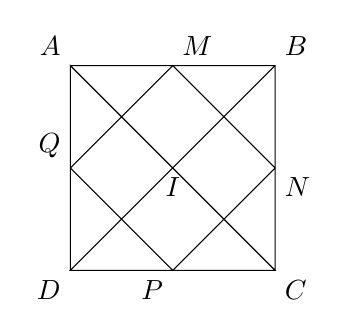
\begin{tikzpicture}[scale=0.65]
	\coordinate[label=above left:$A$] (A) at (0,0);
	\coordinate[label=above right:$B$] (B) at (4,0);
	\coordinate[label=below right:$C$] (C) at (4,-4);
	\coordinate[label=below left:$D$] (D) at (0,-4);
	\coordinate[label=above left:$Q$] (Q) at (0,-2);
	\coordinate[label=above right:$M$] (M) at (2,0);
	\coordinate[label=below right:$N$] (N) at (4,-2);
	\coordinate[label=below left:$P$] (P) at (2,-4);
	\coordinate[label=below:$I$] (I) at (2,-2);
	\draw (A)--(B)--(C)--(D)--(A)--(C)--(D)--(B) (Q)--(M)--(N)--(P)--(Q);	
	\end{tikzpicture}
	}
	}
\end{vd}
\begin{vd}%[9H2K5]
	Cho đường tròn $(O;R)$ và điểm $A$ nằm ngoài $(O)$. Vẽ đường tròn đường kính $OA$, đường tròn này cắt $(O)$ tại hai điểm phân biệt $B$ và $C$. Kẻ $BI$ là đường kính của đường tròn đường kính $OA$, kẻ $BK$ là đường kính của đường tròn $(O)$. Chứng minh rằng
	\begin{listEX}[2]
	\item $AB$, $AC$ là hai tiếp tuyến của $(O)$.
	\item $IK$ là tiếp tuyến của đường tròn $(B;BC)$.
	\end{listEX}	
	\loigiai
	{\immini{
	\vspace*{-0.5cm}
	\begin{enumerate}
	\item $B$ thuộc đường tròn đường kính $OA$ nên $\widehat{ABO}=90^\circ$ mà $B$ thuộc $(O)$ nên $AB$ là tiếp tuyến của $(O)$. Tương tự, ta có $AC$ là tiếp tuyến của $(O)$.
	\item $C$ thuộc đường tròn đường kính $BI$ nên $\widehat{BCI}=90^\circ$. $C$ thuộc đường tròn đường kính $BK$ nên $\widehat{BCK}=90^\circ$. Từ đó suy ra ba điểm $I$, $K$, $C$ thẳng hàng và $IK\perp BC$ tại $C$. Mà $C$ thuộc đường tròn $(B;BC)$ nên $IK$ là tiếp tuyến của $(B;BC)$.
	\end{enumerate}}{\begin{tikzpicture}[line join = round, line cap = round,>=stealth,font=\footnotesize,scale=.85]
	\def\ro{2cm}
	\coordinate[label=right:$O$] (O) at (0,0);
	\coordinate[label=left:$A$] (A) at ($(O)+(180:2.5*\ro)$);
	\draw (O) circle(\ro);
	\coordinate (N) at ($(O)+(10:\ro)$);
	\tkzDefTangent[from=A](O,N)
	\tkzGetPoints{B}{C}
	\node at ($(B)+(110:3mm)$){$B$};
	\node at ($(C)+(-90:3mm)$){$C$};
	\coordinate[label=above:$M$] (M) at ($(A)!.5!(O)$);
	\tkzDrawCircle(M,O)
	\tkzInterLC(B,M)(M,A)
	\tkzGetPoints{I}{}
	\node at ($(I)+(-130:3mm)$){$I$};
	\tkzInterLC(B,O)(O,B)
	\tkzGetPoints{}{K}
	\node at ($(K)+(-80:3mm)$){$K$};
	\tkzMarkSegments[mark=|,size=2](M,A M,O)
	\tkzDrawSegments[add=0 and .3](A,B A,C)
	\tkzDrawSegments(O,B O,C O,A O,K)
	\tkzDrawSegments[dashed](B,C I,K)
	\tkzMarkRightAngles(A,B,O B,C,K)
	\tkzDrawPoints[color=black,fill=black,size=2pt](A,B,C,O,M,I,K)
	\end{tikzpicture}}
	}
\end{vd}
\begin{vd}%[9H2K5]
	Cho tam giác $MNP$ có $\widehat{N}=90^\circ$ và $NP=\dfrac{1}{2}MP=a$. Vẽ đường tròn tâm $P$ tiếp xúc với $MN$ tại $N$. Qua $N$ vẽ tia $Nx$ vuông góc với $MP$ cắt $(P)$ tại điểm thứ hai $Q$ ($Q\ne N$). Chứng minh rằng $MQ$ là tiếp tuyến của $(P)$ và $MNQ$ là tam giác đều.	
	\loigiai
	{\immini{
	Tam giác vuông $MNP$ có $\sin \widehat{NMP}=\dfrac{NP}{MP}=\dfrac{1}{2}$\\ $\Rightarrow \widehat{NMP}=30^\circ$ $\Rightarrow \widehat{MNQ}=90^\circ-30^\circ=60^\circ$.\\
	Ta có hai điểm $N$, $Q$ đối xứng với nhau qua $MP$ nên $\widehat{MQP}=\widehat{MNP}=90^\circ$ và $\widehat{MNQ}=\widehat{MQN}$.\\
	Do đó, $MQ$ là tiếp tuyến của $(P)$ và $MNQ$ là tam giác đều.}{\begin{tikzpicture}[line join = round, line cap = round,>=stealth,font=\footnotesize,scale=.9]
	\def\ro{1.75cm}
	\coordinate[label=above left:$P$] (P) at (0,0);
	\coordinate[label=below:$N$] (N) at ($(P)+(-90:\ro)$);
	\coordinate[label=below:$M$] (M) at ($(N)+(0:2*\ro)$);
	\coordinate[label=above left:$x$] (x) at ($(N)+(60:2.4*\ro)$);
	\tkzInterLC(N,x)(P,N)
	\tkzGetPoints{}{Q}
	\node at ($(Q)+(10:3mm)$){$Q$};
	\tkzLabelSegment[pos=0.6,above](P,M){\tiny $2a$}
	\coordinate (H) at (intersection of N--x and M--P);
	\tkzMarkSegments[mark=|,size=2](H,N H,Q)
	\tkzLabelSegment[pos=0.5,left](P,N){\tiny $a$}
	\tkzMarkRightAngles(N,H,M P,N,M)
	\tkzDrawCircle(P,N)
	\tkzDrawPolygon(M,N,P)
	\tkzDrawSegments(N,x M,P P,Q Q,M)
	\tkzDrawPoints[color=black,fill=black,size=2pt](M,N,P,Q,H)
	\end{tikzpicture}}
	}
\end{vd}
\begin{vd}%[9H2G5]
	Cho tam giác $ABC$ cân tại $A$ và đường tròn $(O)$ có tâm $O$ nằm trên cạnh đáy $BC$; $(O)$ tiếp xúc với các cạnh $AB$, $AC$. Gọi $P$, $Q$ là hai điểm lần lượt nằm trên các cạnh $AB$ và $AC$. Chứng minh rằng $PQ$ tiếp xúc với đường tròn $(O)$ khi và chỉ khi $BP\cdot CQ=\dfrac{BC^2}{4}$.
	\loigiai
	{
	\begin{itemize}
	\item \textbf{\textit{Phần thuận}}\\
	Giả sử $PQ$ tiếp xúc $(O)$ tại $H$. Ta sẽ chứng minh $BP\cdot CQ=\dfrac{BC^2}{4}$. Kí hiệu các tiếp điểm, các góc như hình vẽ. Ta có $\widehat{O_2}=\widehat{O_3}$, $\widehat{O_4}=\widehat{O_5}$ (tính chất hai tiếp tuyến cắt nhau) và $\widehat{O_1}=\widehat{O_6}$ (vì cùng phụ với hai góc bằng nhau). Suy ra $\widehat{O_1}+\widehat{O_2}+\widehat{O_4}=\widehat{O_3}+\widehat{O_5}+\widehat{O_6}=180^\circ:2=90^\circ$. Xét tam giác $OPI$ vuông tại $I$ nên $\widehat{OPI}=90^\circ-\widehat{O_2}$; tam giác $COQ$ có $\widehat{COQ}=\widehat{O_5}+\widehat{O_6}=90^\circ-\widehat{O_3}$. Mà $\widehat{O_2}=\widehat{O_3}$ nên $\widehat{OPI}=\widehat{COQ}$ hay $\widehat{OPB}=\widehat{COQ}$. Do đó $\triangle BPO\equiv \triangle COQ$ (g.g) $\Rightarrow \dfrac{BP}{CO}=\dfrac{BO}{CQ}$ hay $BP\cdot CQ=BO\cdot CO=\dfrac{BC}{2}\cdot \dfrac{BC}{2}=\dfrac{BC^2}{4}$.
	\item \textbf{\textit{Phần đảo}}\\
	Cho $P$, $Q$ tương ứng thuộc hai cạnh $AB$, $AC$ thỏa $BP\cdot CQ=\dfrac{BC^2}{4}$. Ta phải chứng minh $PQ$ tiếp xuc với $(O)$. 
	\immini{
	Giả sử $PQ$ không tiếp xúc với $(O)$ thì ta dựng được $P'Q'$ song song với $PQ$ và tiếp xúc với $(O)$. Theo phần thuận ta có $BP'\cdot CQ'=\dfrac{BC^2}{4}$. Ta xét hai khả năng sau
	\begin{enumerate}[TH1.]
	\item $PQ$ cắt $(O) \colon BP<BP'$ và $CQ<CQ'$ suy ra\\ $BP\cdot CQ<\dfrac{BC^2}{4}$. 
	\item $PQ$ không cắt $(O)\colon BP>BP'$ và $CQ>CQ'$ suy ra $BP\cdot CQ>\dfrac{BC^2}{4}$. Do đó $BP\cdot CQ\ne \dfrac{BC^2}{4}$ (mâu thuẫn với đề bài) $\Rightarrow$ điều giả sử là sai. Vậy $PQ$ tiếp xúc với $(O)$ khi và chỉ khi $BP\cdot CQ=\dfrac{BC^2}{4}$.
	\end{enumerate}	}{
	\begin{tikzpicture}[line join = round, line cap = round,>=stealth,font=\footnotesize,scale=1]
	\def\ro{2}
	\coordinate[label=below:$O$] (O) at (0,0);
	\coordinate[label=above:$H$] (H) at ($(O)+(80:\ro)$);
	\coordinate[label=above:$A$] (A) at ($(O)+(90:2*\ro)$);
	\tkzDefTangent[from=A](O,H)
	\tkzGetPoints{K}{I}
	\node at ($(I)+(160:3mm)$){$I$};
	\node at ($(K)+(10:3mm)$){$K$};
	\tkzDefTangent[at=H](O)
	\tkzGetPoint{d}
	\coordinate[label=left:$P$] (P) at (intersection of H--d and A--I);
	\coordinate[label=right:$Q$] (Q) at (intersection of H--d and A--K);
	\draw let \p1=($(H)-(O)$) in (O) circle ({veclen(\x1,\y1)}); 	
	\coordinate (a) at ($(O)+(0:1)$);
	\coordinate[label=left:$B$] (B) at (intersection of A--I and O--a);
	\coordinate[label=right:$C$] (C) at (intersection of A--K and O--a);
	\tkzLabelAngles[pos=-.4](B,O,I){\tiny $1$}
	\tkzLabelAngles[pos=-.4](I,O,P){\tiny $2$}
	\tkzLabelAngles[pos=-.4](P,O,H){\tiny $3$}
	\tkzLabelAngles[pos=-.4](H,O,Q){\tiny $4$}
	\tkzLabelAngles[pos=-.4](Q,O,K){\tiny $5$}
	\tkzLabelAngles[pos=-.4](K,O,C){\tiny $6$}
	\tkzMarkAngle[arc=l,size=0.6](B,A,O)
	\tkzMarkAngle[arc=l,size=0.6](O,A,C)
	\tkzMarkRightAngles[size=0.15](B,I,O P,H,O Q,K,O)
	\tkzMarkAngle[arc=l,size=0.5,mark=|,mksize=1mm](C,B,A)
	\tkzMarkAngle[arc=l,size=0.5,mark=|,mksize=1mm](A,C,B)
	\tkzDrawPolygon(A,B,C)
	\tkzDrawSegments(P,Q O,A)
	\tkzDrawSegments[dashed](O,I O,H O,P O,Q O,K)
	\end{tikzpicture}
	}
	\end{itemize}	
	}
\end{vd}
%======================
\begin{dang}{Bài toán vận dụng tính chất tiếp tuyến}
	\begin{itemize}
	\item Vận dụng tính chất của tiếp tuyến: Nếu đường thẳng $\Delta$ là tiếp tuyến của $(O)$ tại $A$ thì $\Delta\perp OA$ tại $A$.
	\end{itemize}
\end{dang}
\begin{vd}
	Một thuỷ thủ đang ở trên cột buồm của một con tàu, cách mặt nước biển $10$ m. Biết bán kính Trái Đất là khoảng $6400$ km. Tính tầm nhìn xa tối đa của thuỷ thủ đó (kết quả làm tròn đến hàng phần nghìn).
	\loigiai
	{
	\immini
	{
	Trên hình bên, ta có điểm $B$ biểu diễn vị trí con tàu, điểm $A$ biểu diễn vị trí của thuỷ thủ, điểm $C$ biểu diễn điểm xa nhất mà thuỷ thủ nhìn thấy. Khi đó độ dài đoạn thẳng $AC$ gọi là tầm nhìn xa tối đa từ $A$. Đặt $h=AB, R=OB=OC$. Ta tính $AC$ theo $R$ và $h$. Do $AC$ là tiếp tuyến với $(O;R)$ tại $C$ nên suy ra $AC\perp OC$.\\
	Áp dụng định lí Pythagore trong tam giác $ACO$ vuông tại $C$ ta có:\\
	$AC^2=AO^2-OC^2=(R+h)^2-R^2=2Rh+h^2$.\\
	Suy ra $AC=\sqrt{2Rh+h^2}=\sqrt{2\cdot 6400\cdot 0{,}01+0{,}01^2}\approx 11{,}314\text{(km)}$. \\
	Vậy tầm nhìn xa tối đa của thuỷ thủ đó là khoảng $11{,}314$(km).
	}
	{
	\begin{tikzpicture}[line join = round, line cap = round,>=stealth,font=\footnotesize,scale=1]
	\def\g{50}
	\def\r{1.5}
	\pgfmathsetmacro{\oa}{\r/cos(\g)}
	\path (0,0) coordinate (O) ({90-\g}:\r) coordinate (C) (90:\oa)coordinate (A);
	\draw[name path=c] (O) circle (\r);
	\draw (O)--(C)node[midway,below]{\scriptsize$R$}--(A);
	\draw[name path=a] (O)--(A);
	\path [name intersections={of=c and a,by=B}];
	\foreach\i/\j in{O/-90,C/30,A/90,B/-125}
	\fill[black](\i)circle(1.5pt)node[shift=(\j:2.5mm)]{$\i$};
	\path (B)--(A)node[midway,left]{\scriptsize$h$};
	\pic[draw, angle radius=5pt]{right angle=O--C--A};
	\end{tikzpicture}
	}
	}
\end{vd}
\begin{vd}
	\immini{Cho điểm $M$ nằm ngoài đường tròn $(O; 3 \mathrm{~cm})$ thoả mãn $O M=5 \mathrm{~cm}$. Đường thẳng $M N$ đi qua $M$ và tiếp xúc với đường tròn $(O)$ tại $N$.
	\begin{enumerate}
	\item Tam giác $O M N$ có phải là tam giác vuông hay không? Vì sao?
	\item Tính độ dài đoạn thẳng $M N$.
	\end{enumerate}
	}
	{	\begin{tikzpicture}[>=stealth,line join=round,line cap=round,font=\footnotesize,scale=1]
	\def \r{1.5}
	\path 
	(0,0) coordinate (O)
	(0:\r) coordinate (N)
	($(N)!1.7!90:(O)$) coordinate (M)
	;
	\draw (O)circle(\r);
	\draw (O)--(M)--(N)--(O);
	%\draw (O)--(H)node[pos=0.5,right]{$R$};
	\foreach \x/\y in {N/10,O/90,M/-90}
	\draw[fill=black] (\x) circle (1.1pt) + (\y:0.3cm) node{$\x$};
	\end{tikzpicture}}
	\loigiai{
	\begin{enumerate}
	\item Vì đường thẳng $M N$ tiếp xúc với đường tròn $(O)$ tại $N$ nên $O N \perp M N$.\\ Suy ra tam giác $O M N$ vuông tại $N$.
	\item Áp dụng định lí Py-ta-go cho tam giác $O M N$ vuông tại $N$, ta có\\ $O M^2=O N^2+M N^2$.\\ Suy ra $5^2=3^2+M N^2$.\\	
	Do đó $M N^2=5^2-3^2=25-9=16$.\\
	Vậy $M N=\sqrt{16}=4$ (cm).
	\end{enumerate}
	}
\end{vd}
\begin{vd}
	Cho ba điểm $A, B, C$ thẳng hàng, trong đó $B$ nằm giữa $A$ và $C$. Đường tròn $(O)$ tiếp xúc với đường thẳng $A B$ tại điểm $C$. Chứng minh
	$$
	A O^2+B C^2=B O^2+A C^2 .
	$$
	\loigiai{
	\immini{Vì $AB$ tiếp xúc với $(O)$ tại $C$ nên $AC\perp OC$.\\
	Khi đó áp dụng định lý Py-ta-go cho $\triangle AOC$ vuông tại $C$ ta được \\$AO^2=AC^2+CO^2$ \\
	Suy ra $OC^2=AO^2-AC^2$\, \hfill{(1)}.\\
	Áp dụng định lý Py-ta-go cho $\triangle BOC$ vuông tại $C$ ta được\\ $BO^2=BC^2+CO^2\Rightarrow CO^2=BO^2-BC^2$\, \hfill{(2)}.\\
	Từ $(1)$ và $(2)\Rightarrow AO^2-AC^2=BO^2-BC^2$ \\ Vậy $AO^2+BC^2=BO^2+AC^2$.
	}	{\begin{tikzpicture}[>=stealth,line join=round,line cap=round,font=\footnotesize,scale=0.8]
	\path 
	(0,0) coordinate (A)
	(4,0) coordinate (B)
	($(B)!0.7!180:(A)$) coordinate (C)
	($(C)!0.7!90:(B)$) coordinate (O)
	;
	\draw (O) let \p1=($(O)-(C)$)in circle ({veclen (\x1,\y1)});
	%	\draw (O)circle(\r);
	\draw (B)--(A)--(O)--(C)--(B)--(O);
	%\draw (O)--(H)node[pos=0.5,left]{$R$};
	\foreach \x/\y in {A/180,O/-90,C/90,B/90}
	\draw[fill=black] (\x) circle (1.1pt) + (\y:0.3cm) node{$\x$};
	\draw pic[draw=black,angle radius=5pt] {right angle = A--C--O}; 
	\end{tikzpicture}
	}
	}
\end{vd}
\begin{vd}%[9H2B4]
	Từ điểm $A$ cách $O$ một khoảng $d$ ($d>R$) vẽ tiếp tuyến $AB$ với đường tròn $(O;R)$ ($B$ là tiếp điểm). Tính độ dài đoạn $AB$ theo $d$ và $R$.
	\loigiai{
	\immini{
	Vì $AB$ là tiếp tuyến của $(O)$ tại $B$ nên $AB\perp OB$ tại $B$.\\
	Áp dụng định lí Py-ta-go vào $\triangle AOB$ có
	$$AB=\sqrt{OA^2-OB^2}=\sqrt{d^2-R^2}.$$
	Vậy $AB=\sqrt{d^2-R^2}$. 
	}{
	\begin{tikzpicture}[line join=round, line cap=round]
	\tikzset{label style/.style={font=\footnotesize}}
	\pgfmathsetmacro\h{1.5}
	\tkzDefPoint(0,0){O}
	\tkzDefShiftPoint[O](-90:\h){B}
	\tkzDefShiftPoint[B](0:1.5*\h){A}
	%	\pgfresetboundingbox
	\tkzDrawSegments(O,B O,A)
	\tkzDrawLines[add = 0.7 and 0](B,A)
	\tkzLabelLine[pos=-.85,above,black](B,A){$d$}
	\draw (O) circle (\h);
	\tkzDrawPoints[fill=black](O,A,B)
	\tkzLabelPoints[above](O)
	\tkzLabelPoints[below](B,A)
	\tkzMarkRightAngles(O,B,A)
	\end{tikzpicture}
	}
	}
\end{vd}
\begin{vd}%[9H2Y5]
	Cho đường tròn tâm $O$, bán kính $R=5$cm và một điểm $A$ cách $O$ bằng $13$cm. Kẻ tiếp tuyến $AB$ với đường tròn $(O)$ ($B$ là tiếp điểm). Tính độ dài đoạn $AB$.
	\loigiai
	{\immini{
	Ta có $AB$ là tiếp tuyến của $(O)$ nên $AB\perp OB$. Áp dụng định lí Py-ta-go vào tam giác vuông $ABO$, ta có\\ $AB^2=OA^2-OB^2=13^2-5^2=144$ $\Rightarrow AB=12$.\\ Vậy $AB=12$cm.}{
	\vspace*{-3mm}
	\begin{tikzpicture}[line join = round, line cap = round,>=stealth,font=\footnotesize,scale=.75]
	\def\ro{2cm}
	\coordinate[label=below:$O$] (O) at (0,0);
	\coordinate[label=below:$A$] (A) at ($(O)+(180:2.5*\ro)$);
	\coordinate (M) at ($(O)+(0:\ro)$);
	\tkzDefTangent[from=A](O,M)
	\tkzGetPoints{B}{}
	\node at ($(B)+(90:3mm)$){$B$};
	\tkzDrawCircle(O,M)
	\tkzLabelSegment[below,pos=0.5](A,O){\tiny $13$}
	\tkzLabelSegment[right,pos=0.5](O,B){\tiny $5$}
	\tkzDrawSegments(A,O O,B A,B)
	\tkzMarkRightAngles(A,B,O)
	\tkzDrawPoints[color=black,fill=black,size=2pt](A,O,B)
	\end{tikzpicture}}
	}
\end{vd}
\begin{vd}%[9H2K4]
	Cho đường tròn $(O;5\text{ cm})$ và dây $AB=8$ cm. Một tiếp tuyến của $(O)$ song song với $AB$ cắt tia $OA$ tại $E$, cắt tia $OB$ tại $F$. Tính độ dài đoạn $EF$.
	\loigiai{
	\immini{
	Gọi $C$ là tiếp điểm của tiếp tuyến $EF$ với $(O)$, $H$ là giao điểm của $OC$ với $AB$. Ta có $OC\perp EF$ tại $C$ mà $AB\perp EF$ nên $OC\perp AB$ tại $H$.
	$\Rightarrow HA=HB=\dfrac{1}{2}AB=4\text{ cm}$.\\
	Áp dụng định lí Py-ta-go vào $\triangle OHA$. ta có
	$$OH=\sqrt{OA^2-AH^2}=\sqrt{5^2-4^2}=3\text{ cm}.$$
	Ta có $AB\parallel EF$ nên theo định lí Ta-lét có
	$$\dfrac{AB}{EF}=\dfrac{OB}{OF}=\dfrac{OH}{OC}=\dfrac{3}{5}\Rightarrow EF=\dfrac{5}{3}\cdot AB=\dfrac{5\cdot8}{3}=\dfrac{40}{3}\text{ cm}.$$
	}{
	\begin{tikzpicture}[line join=round, line cap=round]
	\tikzset{label style/.style={font=\footnotesize}}
	\pgfmathsetmacro\h{2}
	\tkzDefPoint(0,0){O}
	\tkzDefShiftPoint[O](90:\h){C}
	\coordinate (H) at ($(O)!3/5!(C)$);
	\tkzDefLine[orthogonal=through C](O,C)\tkzGetPoint{c}
	\tkzDefLine[orthogonal=through H](O,C)\tkzGetPoint{h}
	\tkzInterLC(H,h)(O,C)\tkzGetPoints{B}{A}
	\tkzInterLL(O,A)(c,C)\tkzGetPoint{E}
	\tkzInterLL(O,B)(c,C)\tkzGetPoint{F}
	\pgfresetboundingbox
	\draw (O)--(E)--(F)--cycle (A)--(B) (O)--(C);
	\draw (O) circle (\h);
	\tkzDrawPoints[fill=black](O,A,B,E,C,F,H)
	\tkzLabelPoints[above](E,C,F)
	\tkzLabelPoints[below](O)
	\tkzLabelPoints[left](A)
	\tkzLabelPoints[below left](H)
	\tkzLabelPoints[right](B)
	\tkzMarkRightAngles[size=0.15](O,C,F O,H,B)
	\tkzLabelSegment[pos=0.7,yshift=-0.5cm](O,B){$5$}
	\tkzLabelSegments[pos=0.5](A,H H,B){$4$}
	\end{tikzpicture}
	}
	}
\end{vd}
\begin{vd}%[9H2K4]
	Cho hai đường tròn đồng tâm $(O;R_1)$ và $(O;R_2)$ $(0<R_1<R_2)$. Từ điểm $M$ nằm ngoài $(O;R_2)$, ta vẽ $MA$ là tiếp tuyến của $(O;R_1)$, $MB$ là tiếp tuyến của $(O;R_2)$ (với $A$, $B$ là các tiếp điểm). Đường trung trực của đoạn $AB$ cắt $OM$ tại $I$. Tính tỉ số $\dfrac{MI}{MO}$.
	\loigiai
	{
	\immini{
	Gọi $I'$ là trung điểm của $OM$. Vì $MA$ là tiếp tuyến của $(O;R_1)$ nên $MA\perp OA$ tại $A$ hay $\widehat{OAM}=90^\circ$. Xét $\triangle OAM$ có $\widehat{OAM}=90^\circ$, $AI'$ là trung tuyến ứng với cạnh huyền $MO$ nên $AI'=\dfrac{1}{2}OM$.\\
	Tương tự ta có $BI'=\dfrac{1}{2}OM\Rightarrow AI'=BI'=\dfrac{1}{2}OM$ $\Rightarrow I'$ thuộc đường trung trực $d$ của đoạn $AB$	 $\Rightarrow I'\equiv I\Rightarrow \dfrac{MI}{MO}=\dfrac{MI'}{MO}=\dfrac{1}{2}$.}{\begin{tikzpicture}[line join=round, line cap=round]
	\tikzset{label style/.style={font=\footnotesize}}
	\pgfmathsetmacro\h{1.5}
	\pgfmathsetmacro\ra{\h}
	\pgfmathsetmacro\rb{1.8*\h}
	\tkzDefPoint(0,0){O}
	\tkzDefShiftPoint[O](0:2.5*\h){M}
	\tkzDefTangent[from with R=M](O,\ra cm)\tkzGetPoints{a}{A}
	\tkzDefTangent[from with R=M](O,\rb cm)\tkzGetPoints{b}{B}
	\coordinate (ab) at ($(A)!1/2!(B)$);
	\tkzDefLine[orthogonal=through ab](A,B)\tkzGetPoint{d}
	\tkzInterLL(O,M)(ab,d)\tkzGetPoint{I}
	\pgfresetboundingbox
	\draw (O)--(A)--(B)--cycle (O)--(M);
	\draw[dashed] (A)--(I)--(B);
	\tkzDrawLines[add = 0 and 0.4](M,A M,B)
	\tkzDrawLines[add = 0.3 and 0.6](ab,I)
	\tkzLabelLine[pos=1.6,above,black](ab,I){$d$}
	\draw (O) circle (\ra);
	\draw (O) circle (\rb);
	\tkzDrawPoints[fill=black](O,A,B,I,M)
	\tkzLabelPoints[above](A,B)
	\tkzLabelPoints[below](O,I,M)
	\tkzMarkRightAngles[size=0.15](O,A,M O,B,M)
	\tkzMarkSegments[pos=0.5,mark=|](ab,A ab,B)
	\node[above right]at(I){$I'$};
	\end{tikzpicture}}
	}
\end{vd}
\begin{vd}%[9H2K5]
	Cho đường tròn $(O)$, bán kính $R=3$, dây $MN$ vuông góc với bán kính $OP$ tại trung điểm của $OP$. Tiếp tuyến tại $M$ của $(O)$ cắt tia $OP$ tại $I$. Tính độ dài $MI$.
	\loigiai{
	\immini{
	Gọi $H$ là giao điểm của $MN$ và $OP$. \\Ta có $MH=\sqrt{OM^2-OH^2}=\sqrt{3^2-\left(\dfrac{3}{2}\right)^2}=\dfrac{3\sqrt{3}}{2}$.\\
	Do đó, $\sin \widehat{OMH}=\dfrac{OH}{OM}=\dfrac{1}{2}$ $\Rightarrow \widehat{OMH}=30^\circ$ $\Rightarrow \widehat{MIO}=30^\circ$. \\Từ đó suy ra $MI=2MH=3\sqrt{3}$.}{
	\begin{tikzpicture}[line join = round, line cap = round,>=stealth,font=\footnotesize,scale=0.7]
	\def\ro{3cm}
	\coordinate[label=below:$O$] (O) at (0,0);
	\coordinate[label=below:$I$] (I) at ($(O)+(180:5.196)$);
	\coordinate (A) at ($(O)+(0:\ro)$);
	\tkzDefTangent[from=I](O,A)
	\tkzGetPoints{M}{N}
	\node at ($(M)+(90:3mm)$){$M$};
	\node at ($(N)+(-90:3mm)$){$N$};
	\tkzDrawCircle(O,A)
	\coordinate (H) at (intersection of M--N and I--O);
	\node at ($(H)+(-50:3mm)$){$H$};
	\tkzInterLC(I,O)(O,A)
	\tkzGetPoints{P}{}
	\node at ($(P)+(210:3mm)$){$P$};
	\tkzMarkSegments[mark=|,size=2](P,H H,O)
	\tkzMarkRightAngles(M,H,O I,M,O)
	\tkzDrawSegments(I,M I,O M,N O,M)
	\tkzDrawPoints[color=black,fill=black,size=2pt](O,I,M,N,P,H)
	\end{tikzpicture}
	}
	}
\end{vd}
%==================
\begin{dang}{Bài toán vận dụng tính chất của hai tiếp tuyến cắt nhau}
\end{dang}	
%%==========Thực hành 4
\begin{vd}
	\immini
	{
	Tìm giá trị của $x$.
	}
	{
	\begin{tikzpicture}[line join = round, line cap = round,>=stealth,font=\footnotesize,scale=1]
	\def\r{1.5}
	\path (0,0) coordinate (D) (3.5,0) coordinate (B) ($(D)!.5!(B)$)coordinate (X);
	\draw[name path=c] (D) circle (\r);
	\path[name path=c'] (X) let \p1=($(X)-(D)$) in circle ({veclen(\x1,\y1)});
	\path[name intersections={of=c and c',by={A,C}}];
	\foreach\i/\j in{D/180,B/0,A/90,C/-90}
	\fill[black](\i)circle(1.5pt)node[shift=(\j:2.5mm)]{$\i$};
	\draw (A)--(B)node[midway,above,sloped]{$4x-9$}--(C)node[midway,below ,sloped]{$15$}--(D)--cycle;
	\pic[draw, angle radius=5pt]{right angle=D--A--B};
	\pic[draw, angle radius=5pt]{right angle=D--C--B};
	\end{tikzpicture}
	}
	\loigiai{
	Vì $AB$ và $BC$ là hai tiếp tuyến của $(O)$ nên $AB=BC$.\\
	Suy ra $4x-9=15\Rightarrow 4x=24 \Rightarrow x=6$
	}
\end{vd}
%%==========Vận dụng 3
\begin{vd}
	\immini
	{
	Bánh đà của một động cơ được thiết kế có dạng là một đường tròn tâm $O$, bán kính $15$ cm được kéo bởi một dây curoa. Trục của mô tơ truyền lực được biểu diễn bời điểm $M$. Cho biêt khoảng cách $OM$ là $35$ cm.
	\begin{listEX}[1]
	\item Tính độ dài của hai đoạn dây curoa $MA$ và $MB$ (kết quả làm tròn đến hàng phần mười).
	\item Tính số đo $\widehat{AMB}$ tạo bởi hai tiếp tuyến $AM$, $BM$ và số đo $\widehat{AOB}$ (kết quả làm tròn đến phút).
	\end{listEX}
	}
	{
	\begin{tikzpicture}[line join = round, line cap = round,>=stealth,font=\footnotesize,scale=1]
	\def\r{1.5}
	\path (0,0) coordinate (O) (0,-3) coordinate (M) ($(O)!.5!(M)$)coordinate (X);
	\draw[name path=c] (O) circle (\r);
	\path[name path=c'] (X) let \p1=($(X)-(O)$) in circle ({veclen(\x1,\y1)});
	\path[name intersections={of=c and c',by={A,B}}];
	\foreach\i/\j in{O/90,A/-135,B/-45,M/-90}
	\fill[black](\i)circle(1.5pt)node[shift=(\j:2.5mm)]{$\i$};
	\draw (A)--(M)--(B)--(O)--cycle;
	\pic[draw, angle radius=5pt]{right angle=O--A--M};
	\pic[draw, angle radius=5pt]{right angle=O--B--M};
	\end{tikzpicture}
	}
	\loigiai{
	\begin{enumerate}
	\item Xét $\triangle AMO$ vuông tại $A$ ta có:\\
	$
	\begin{aligned}
	&MA^2+OA^2=OM^2 \text {(định lí Pythagore)}\\ 
	&\Rightarrow MA^2+15^2=35^2 
	\Rightarrow MA^2+225=1225 
	\Rightarrow MA^2=1000 
	\Rightarrow MA=10 \sqrt{10} 
	\Rightarrow MA=31{,}2(\text{cm})
	\end{aligned}
	$\\
	Mà $MA=MB$ nên $MB=31{,}2(\text{cm})$.
	\item Xét $\triangle AMO$ vuông tại $E$ ta có:\\
	$
	\begin{aligned}
	\sin \widehat{OMA}=\dfrac{OA}{OM} \text {(TSLG)} 
	\Rightarrow \sin \widehat{OMA}=\dfrac{15}{35}=\dfrac{3}{7} \Rightarrow \widehat{OMA} \approx 25^{\circ} 23^{\prime}
	\end{aligned}
	$\\
	Xét $(O)$, ta có:\\
	Hai tiếp tuyến $MA, MB$ cắt nhau tại $M$ (gt)\\
	$\Rightarrow MO$ là tia phân giác của $\widehat{AMB}$\\
	$ \Rightarrow \widehat{AMB}=2 \widehat{OMA}=2\cdot25^{\circ} 23^{\prime}=50^{\circ} 46^{\prime}$.
	\end{enumerate}
	}
\end{vd}
\begin{vd}
	Cho điểm $A$ nằm ngoài đường tròn $(O;R)$. Vẽ đường tròn đường kính $AO$ cắt đường tròn $(O;R)$ tại hai điểm $B$ và $C$.
	\begin{listEX}[1]
	\item Chứng minh $AB$ và $AC$ là các tiếp tuyến của đường tròn $(O;R)$. 
	\item Chứng minh $AB=AC$.
	\item Xác định tia phân giác của $\widehat{BAC}$ và $\widehat{BOC}$.
	\end{listEX}
	\loigiai{
	\begin{enumerate}
	\item Gọi $M$ là trung điểm của $AO$.
	\immini{
	Ta có $M$ là tâm của đường tròn đường kính $AO$, suy ra $MB=MC=\dfrac{AO}{2}$.\\
	Do đó, tam giác $ABO$ vuông tại $B$ và tam giác $ACO$ vuông tại $C$. \\
	Vì $AB$ vuông góc với bán kính $OB$ tại $B$ và $AC$ vuông góc với bán kính $OC$ tại $C$ nên $AB$ và $AC$ là hai tiếp tuyến với đường tròn $(O)$ tại $B$ và $C$.
	\item Giao điểm $A$ của hai tiếp tuyến $AB, AC$ cách đều hai tiếp điểm $B$ và $C$ nên $AB=AC$.
	\item Hai tiếp tuyến tại $B$ và $C$ của đường tròn $(O)$ cắt nhau tại $A$, suy ra tia $AO$ là phân giác của $\widehat{BAC}$ và tia $OA$ là phân giác của $\widehat{BOC}$.}{
	\begin{tikzpicture}[line join = round, line cap = round,>=stealth,font=\footnotesize,scale=1]
	\def\r{1.5}
	\path (0,0) coordinate (O) (-4,0) coordinate (A) ($(A)!.5!(O)$)coordinate (M);
	\draw[name path=c] (O) circle (\r);
	\draw[name path=c'] (M) let \p1=($(M)-(O)$) in circle ({veclen(\x1,\y1)});
	\path[name intersections={of=c and c',by={B,C}}];
	\foreach\i/\j in{B/90,C/-90,A/180,O/0,M/-90}
	\fill[black](\i)circle(1.5pt)node[shift=(\j:2.5mm)]{$\i$};
	\draw (A)--(B)--(O)--(C)--cycle (M)--(B)--(O)--(C)--cycle (A)--(O);
	\pic[draw, angle radius=5pt]{right angle=A--B--O};
	\pic[draw, angle radius=5pt]{right angle=A--C--O};
	\path ($(A)!.5!(M)$)node{$|$} ($(O)!.5!(M)$)node{$|$};
	\end{tikzpicture}
	}
	\end{enumerate}
	}
\end{vd}
%%==========Thực hành 3
\begin{vd}
	Cho điểm $M$ nằm ngoài đường tròn $(I;6\text{cm})$ và $ME$, $MF$ là hai tiếp tuyến của đường tròn này tại $E$ và $F$. Cho biết $\widehat{EMF}=60^{\circ}$.
	\begin{listEX}[2]
	\item Tính số đo $\widehat{EMI}$ và $\widehat{EIF}$. 
	\item Tính độ dài $MI$.
	\end{listEX}
	\loigiai{
	\begin{listEX}[1]
	\item
	Xét $(O)$, ta có:
	Hai tiếp tuyến $ME, MF$ cắt nhau tại $M (gt)$
	\immini{
	$\Rightarrow MI$ là tia phân giác của $\widehat{EMF}$
	$ \Rightarrow \widehat{EMI}=\dfrac{\widehat{EMF}}{2}=\dfrac{60^{\circ}}{2}=30^{\circ}.
	$
	Xét tứ giác $IEMF$, ta có:\\
	$ \widehat{EIF}+\widehat{FM}+\widehat{EMF}+\widehat{MEI}=360^{\circ} \text {(tổng $4$ góc trong một tứ giác)}$ \\
	$\Rightarrow\widehat{EIF}+90^{\circ}+60^{\circ}+90^{\circ}=360^{\circ} $\\
	$\Rightarrow \widehat{EIF}=120^{\circ}$
	\item
	Xét $\triangle EMI$ vuông tại $E$ ta có:\\
	$ \sin \widehat{EMI}=\dfrac{IE}{IM}$(TSLG) \\
	$ \Rightarrow \sin 30^{\circ}=\dfrac{6}{IM} \Rightarrow \dfrac{1}{2}=\dfrac{6}{IM} \Rightarrow IM=12$ (cm).}{
	\begin{tikzpicture}[line join = round, line cap = round,>=stealth,font=\footnotesize,scale=1]
	\def\r{2}
	\pgfmathsetmacro{\a}{\r/sin(30)}
	\path (0,0) coordinate (I) (\a,0) coordinate (M)
	($(I)!.5!(M)$) coordinate (X);
	\path[name path=c'] (X) let \p1=($(X)-(I)$) in circle ({veclen(\x1,\y1)});
	\draw[name path=c] (I) circle (\r);
	\path[name intersections={of=c and c',by={E,F}}];
	\foreach\i/\j in{E/90,F/-90,I/180,M/0}
	\fill[black](\i)circle(1.5pt)node[shift=(\j:2.5mm)]{$\i$};
	\draw (M)--(E)--(I)--(F)--cycle (E)--(F) (M)--(I);
	\draw pic[draw=black,angle radius=5pt] {right angle = M--E--I}; 
	\draw pic[draw=black,angle radius=5pt] {right angle = M--F--I};
	\end{tikzpicture}
	}
	\end{listEX}
	}
\end{vd}
\begin{vd}
	Một chiếc gương có dạng hình tròn được treo bằng hai sợi dây không dãn, mỗi sợi dây đều tiếp xúc với gương (Hình a). Biết tổng độ dài hai dây treo là $6$ dm và góc giữa hai sợi dây là $60^{\circ}$. Hỏi bán kính của chiếc gương là bao nhiêu decimét (làm tròn kết quả đến hàng phần trăm)?
	\begin{center}
	\begin{tabular}{cc}
	\includegraphics[scale=0.65]{images/9C5-3-Vd4}& 
	\begin{tikzpicture}[>=stealth,line join=round,line cap=round,font=\footnotesize,scale=0.8]
	\def \r{2}
	\path 
	(0,0) coordinate (O)
	(0:\r) coordinate (M)
	(25:\r) coordinate (B)
	(155:\r) coordinate (A)
	($(A)!3!90:(O)$) coordinate (x)
	($(B)!3!-90:(O)$) coordinate (y)
	(intersection of A--x and B--y) coordinate (M)
	;
	\draw (O)circle(\r);
	\draw (M)--(B)--(O)--(A)--(M)--(O);
	\foreach \x/\y in {M/90,O/-90,A/180,B/0}
	\draw[fill=black] (\x) circle (1.1pt) + (\y:0.3cm) node{$\x$};
	\end{tikzpicture}\\
	Hình a& Hình b\\
	\end{tabular}
	\end{center}
	\loigiai{
	Giả sử chiếc gương được minh hoạ bởi đường tròn $(O)$, hai sợi dây treo là hai tiếp tuyến cắt nhau $M A$, $M B$ của đường tròn $(O)$, trong đó $M A+M B=6$ dm và $\widehat{A M B}=60^{\circ}$ (Hình b).\\	
	Vì $M A, M B$ là các tiếp tuyến của $(O)$ nên $M A=M B$ và $\widehat{O M A}=\widehat{O M B}$, suy ra $M A=3 \mathrm{dm}$ và $\widehat{O M A}=30^{\circ}$.\\
	Xét tam giác $O M A$ vuông tại $A$, ta có
	$
	O A=M A \cdot \tan \widehat{O M A}=3 \cdot \tan 30^{\circ}=3 \cdot \dfrac{\sqrt{3}}{3} \approx 1{,}73$ (dm).\\ 	
	Vậy bán kính của chiếc gương là khoảng $1{,}73$ dm.
	}
\end{vd}
\begin{vd}
	Cho đường tròn $(O; R)$ và điểm $M$ nằm ngoài đường tròn. Hai đường thẳng $c$, $d$ qua $M$ lần lượt tiếp xúc với $(O)$ tại $A$, $B$. Biết $\widehat{A M B}=120^{\circ}$. Chứng minh $A B=R$.
	\loigiai{
	\immini{Đường thẳng $c$, $d$ qua $M$ lần lượt tiếp xúc với $(O)$ tại $A$, $B$ nên $MB\perp OB$ và $MA\perp OA$.\\
	Đường thẳng $c$, $d$ là hai tiếp tuyến cắt nhau tại $M$.\\
	Khi đó $OM$ là tia phân giác của góc $\widehat{AOB}$\\
	$MO$ là tia phân giác của góc $\widehat{AMB}\Rightarrow \widehat{BMO}=\widehat{AMO}=60^{\circ}$.\\
	Xét $\triangle OMB$ có $\widehat{BOM}+\widehat{OMB}+\widehat{MBO}=180^{\circ}\Rightarrow OBM=30^{\circ}$.\\
	$OM$ là tia phân giác của góc $\widehat{AOB}$ nên $\widehat{AOM}=\widehat{MOB}=30^{\circ}$.\\
	Xét $\triangle AOB$ có $\heva{&OA=OB\\&\widehat{AOB}=60^{\circ}}$ suy ra $\triangle AOB$ đều.\\ Do đó $AB=R$.	
	}
	{\begin{tikzpicture}[>=stealth,line join=round,line cap=round,font=\footnotesize,scale=1]
	\def \r{2}
	\clip (-\r-0.1,-\r-0.5) rectangle (\r+1,\r+0.5);
	\path 
	(0,0) coordinate (O)
	(0:\r) coordinate (M)
	(30:\r) coordinate (B)
	(-30:\r) coordinate (A)
	($(A)!3!90:(O)$) coordinate (x)
	($(B)!3!-90:(O)$) coordinate (y)
	(intersection of A--x and B--y) coordinate (M)
	($(A)!1!180:(M)$) coordinate (c)
	($(B)!1!180:(M)$) coordinate (d)
	;
	\draw (O)circle(\r);
	\draw (M)--(B)--(O)--(A)--(M)--(O)(B)--(d) (A)--(c);
	\foreach \x/\y in {M/0,O/-90,A/-90,B/0}
	\draw[fill=black] (\x) circle (1.1pt) + (\y:0.3cm) node{$\x$};
	\foreach \x/\y in {d/90,c/-90}
	\draw[fill=black] (\x) circle (0pt) + (\y:0.3cm) node{$\x$};
	\end{tikzpicture}}
	}
\end{vd}
\begin{vd}
	Cho hai tiếp tuyến $P A$ và $P B$ của đường tròn $(O; R)$ ( $A$ và $B$ là hai tiếp điểm).
	\begin{listEX}[2]
	\item Chứng minh rằng $O P \perp A B$;
	\item Tính $P A$ và $P B$, biết $R=2 \mathrm{~cm}$ và $P O=4 \mathrm{~cm}$.
	\end{listEX}
	\loigiai{
	\begin{enumerate}
	\item 
	Do $O A$ và $O B$ là hai tiếp tuyến cắt nhau của $(O)$ nên ta có $O P$ là tia phân giác của góc $A O B$. Trong tam giác cân $A O B\ (O A=O B)$, đường phân giác $O P$ cũng là đường cao nên ta có $O P \perp A B$.
	\item Tam giác $O A P$ có $\widehat{O A P}=90^{\circ}$ (do $P A$ tiếp xúc với đường tròn $(O)$ tại $A$) và $O A=R=2 \mathrm{~cm}$ và $O P=4 \mathrm{~cm}$ (giả thiết).
	\immini{
	Áp dụng định lí Pythagore vào tam giác vuông $O A P$ ta có 
	$$A P^{2}+O A^{2}=O P^{2}.$$
	Từ đó suy ra $A P^{2}=O P^{2}-O A^{2}=4^{2}-2^{2}=12$.\\
	Vậy $A P=\sqrt{12}=2 \sqrt{3}$ (cm).\\
	Theo tính chất của hai tiếp tuyến cắt nhau, ta cũng có 
	$$B P=A P=2 \sqrt{3} \mathrm{~cm}.$$
	}{
	\begin{tikzpicture}[scale=0.95, font=\footnotesize, line join=round, line cap=round, >=stealth]
	\coordinate[label=right:$O$] (O) at (0,0);
	\coordinate[label=above left:$M$] (M) at (-2,0);
	\coordinate[label=left:$P$] (C) at (-4,0);
	\draw[name path=circleO] (O) circle[radius=2cm];
	\path[name path=circleX] let \p1=($(O)-($(O)!.5!(C)$)$) in ($(O)!.5!(C)$) circle ({veclen(\x1,\y1)});
	\path[name intersections={of= circleX and circleO}] coordinate (A) at (intersection-1) coordinate (B) at (intersection-2);
	\path (intersection of A--B and C--O) coordinate (D) node[below left]{$H$}; 
	\draw (C)--(A)node[above]{$A$}--(O)--(B)node[below]{$B$}--(C)--(O) (M)--(A)--(B);
	\foreach \diem in {O,A,B,C,D,M}\fill (\diem)circle(1pt); 
	\draw pic[angle radius=2mm,draw=black] {right angle =O--A--C};
	\draw pic[angle radius=2mm,draw=black] {right angle =O--B--C};
	\end{tikzpicture}
	}
	\end{enumerate}
	}
\end{vd}
%================
\begin{dang}{Chứng minh một số tính chất và hệ thức hình học}
	\begin{itemize}
	\item Chứng minh hai đường thẳng vuông góc nhờ tính chất của tiếp tuyến.
	\item Chứng minh hai đoạn thẳng bằng nhau, hai góc bằng nhau nhờ tính chất hai tiếp tuyến cắt nhau.
	\item Áp dụng định lý Py-ta-go, hệ thức lượng trong tam giác vuông để chứng minh đẳng thức về đoạn thẳng, diện tích, $\cdots$
	\end{itemize}
\end{dang}	
\begin{vd}%[9H2B6]
	Cho đường tròn $(O;R)$ và một điểm $A$ nằm ngoài $(O)$. Từ $A$ kẻ các tiếp tuyến $AB$, $AC$ với $(O)$. Vẽ đường kính $CD$. Chứng minh rằng
	\begin{listEX}[2]
	\item $OA\perp BC$;
	\item $BD\parallel OA$.
	\end{listEX}	
	\loigiai{
	\immini{\vspace*{-4mm}
	\begin{enumerate}
	\item Ta có $AB$, $AC$ là tiếp tuyến của $(O)$ nên $AB=AC$. \tagEX{1}
	$B$, $C$ thuộc $(O)$ nên $OB=OC=R$. \tagEX{2}
	Từ $(1)$ và $(2)$ suy ra $A$ và $O$ cách đều hai đầu đoạn thẳng $BC$ nên $AO$ là đường trung trực của đoạn $BC$. Suy ra $OA\perp BC$.
	\item Gọi $I$ là giao điểm của $OA$ và $BC$, vì $OA$ là trung trực của $BC$ nên $I$ là trung điểm của $BC$. Do đó $OI$ là đường trung bình của tam giác $BCD$. Suy ra $BD\parallel OI$ hay $OA\parallel BD$. (có thể chứng minh bằng cách chỉ ra $BD$, $OA$ cùng vuông góc với $BC$).
	\end{enumerate}	
	}{
	\begin{tikzpicture}[line join = round, line cap = round,>=stealth,font=\footnotesize,scale=.8]
	\def\ro{2cm}
	\coordinate[label=right:$O$] (O) at (0,0);
	\coordinate[label=left:$A$] (A) at ($(O)+(180:2.5*\ro)$);
	\draw (O) circle(\ro);
	\coordinate (N) at ($(O)+(10:\ro)$);
	\tkzDefTangent[from=A](O,N)
	\tkzGetPoints{B}{C}
	\node at ($(B)+(110:3mm)$){$B$};
	\node at ($(C)+(-90:3mm)$){$C$};
	\coordinate[label=above:$D$](D) at ([rotate around={180:(O)}]C);
	\coordinate (c) at ($(A)!1.2!(C)$);
	\coordinate[label=above left:$I$] (I) at (intersection of B--C and A--O);
	\tkzDrawSegments[add=0 and .3](A,B A,C)
	\tkzDrawSegments(O,B O,C O,A B,C C,D B,D)
	\tkzMarkRightAngles(A,B,O D,C,c B,I,O)
	\tkzDrawPoints[color=black,fill=black,size=2pt](A,B,C,O,D,I)
	\end{tikzpicture}
	}
	}
\end{vd}
\begin{vd}%[9H2G6]
	Cho tam giác $ABC$ vuông tại $A$. Đường tròn nội tiếp tam giác $ABC$ tiếp xúc cạnh $BC$ tại $D$. Chứng minh rằng $S_{\triangle ABC}=BD\cdot DC$.	
	\loigiai
	{\immini{ \vspace*{-0.5cm}
	\begin{itemize}
	\item Đặt $BC=a$, $AC=b$, $AB=c$. Gọi $I$ là tâm đường tròn nội tiếp tam giác $ABC$ ($I$ là giao điểm của ba đường phân giác trong của tam giác $ABC$). Gọi $E$, $F$ là các điểm tiếp xúc của $(I)$ với $AC$, $AB$. Theo tính chất hai tiếp tuyến cắt nhau, ta có $BD=BF$, $CD=CE$, $AE=AF$.
	\item Mặt khác, ta lại có
	\allowdisplaybreaks
	\begin{eqnarray*}
	BD+BF	& =& AB+BC-(AF+CD)\Leftrightarrow 2BD=BA+BC-(AE+CE)\\
	&\Leftrightarrow & 2BD=c+a-b\Leftrightarrow BD=\dfrac{a+c-b}{2}=\dfrac{a-(b-c)}{2} 
	\end{eqnarray*}
	\end{itemize}	}{\begin{tikzpicture}[line join = round, line cap = round,>=stealth,font=\footnotesize,scale=1.2]
	\tkzInit[xmin=-.5,ymin=-.5,xmax=4.5,ymax=2.25]
	\tkzClip
	\coordinate[label=below left:$B$] (B) at (0,0);
	\coordinate[label=below right:$C$] (C) at ($(B)+(0:4)$);
	\tkzDefTriangle[two angles= 55 and 35](B,C)
	\tkzGetPoint{A}
	%\pgfresetboundingbox
	\node at ($(A)+(90:3mm)$){$A$};
	\tkzDefCircle[in](A,B,C)
	\tkzGetPoint{I}
	\node at ($(I)+(-10:3mm)$){$I$};
	\coordinate[label=left:$F$] (F) at ($(A)!(I)!(B)$);
	\coordinate[label=right:$E$] (E) at ($(A)!(I)!(C)$);
	\coordinate[label=below:$D$] (D) at ($(B)!(I)!(C)$);
	\tkzDrawPolygon(A,B,C)
	\tkzDrawCircle(I,E)
	\tkzDrawSegments[dashed](I,D)
	\tkzDrawSegments[dashed,add=0 and .72](A,I)
	\tkzDrawSegments[dashed,add=0 and .45](B,I)
	\tkzDrawSegments(I,F I,E)
	\tkzMarkRightAngles[size=.15](I,D,B B,A,C)
	\tkzDrawPoints[color=black,fill=black,size=2pt](A,B,C,E,F,D,I)
	\end{tikzpicture}}
	\begin{itemize}
	\item Tương tự, ta co $DC=\dfrac{a+(b-c)}{2}$.
	\item Do đó
	\allowdisplaybreaks
	\begin{eqnarray*}
	BD\cdot	DC&= & \dfrac{a-(b-c)}{2}\cdot\\
	&\Leftrightarrow & \dfrac{a+(b-c)}{2}=\dfrac{a^2-(b-c)^2}{4} \\
	&= & \dfrac{\left[a^2-(b^2+c^2)\right]+2bc}{4}=\dfrac{2bc}{4}=\dfrac{bc}{2} (\text{ vì } a^2=b^2+c^2)
	=S_{\triangle ABC}
	\end{eqnarray*}
	\end{itemize}
	}
\end{vd}
\begin{vd}%[9H2G6]
	Từ một điểm $A$ nằm ngoài đường tròn $(O;R)$ vẽ hai tiếp tuyến $AB$, $AC$ với đường tròn $(O)$ ($B$, $C$ là các tiếp điểm). Gọi $H$ là chân đường vuông góc vẽ từ $B$ xuống đường kính $CD$ của $(O)$. Chứng minh rằng $IB=IH$ với $I$ là giao điểm của $AD$ và $BH$.
	\loigiai
	{\immini{ \vspace*{-0.5cm}
	\begin{itemize}
	\item Gọi $E$ là giao điểm của $CA$ và $DB$. Vì $AB$, $AC$ là các tiếp tuyến của $(O)$ nên ta có $AB=AC$, suy ra tam giác $ABC$ cân tại $A$ $\Rightarrow \widehat{ACB}=\widehat{ABC}$.
	\item Vì $B$ thuộc đường tròn đường kính $CD$ nên $\widehat{CBD}=90^\circ\Rightarrow \widehat{CBE}=90^\circ$.
	\item Do đó $\widehat{AEB}+\widehat{BCA}=\widehat{ABE}+\widehat{ABC}=90^\circ$. Mà $\widehat{ACB}=\widehat{ABC}$ nên $\widehat{AEB}=\widehat{ABE}$ $\Rightarrow$ tam giác $ABE$ cân tại $A$ $\Rightarrow AE=AB\Rightarrow AB=AC=AE$.
	\item Vì $AC$ là tiếp tuyến của $(O)$ nên $AC\perp CD$ $\Rightarrow AC \parallel BH$ (vì cùng vuông góc với $CD$).\\
	Xét tam giác $ACD$ có $IH\parallel AC$ nên $\dfrac{IH}{AC}=\dfrac{DI}{DA}$.\tagEX{1}
	Xét tam giác $ADE$ có $IB\parallel AE$ nên $\dfrac{IB}{AE}=\dfrac{DI}{DA}$.\tagEX{2}
	\item Từ $(1)$ và $(2)$ suy ra $\dfrac{IH}{AC}=\dfrac{IB}{AE}\Rightarrow IH=IB$ (vì $AC=AE$).
	\end{itemize}
	}{\begin{tikzpicture}[line join = round, line cap = round,>=stealth,font=\footnotesize,scale=1]
	\def\ro{2cm}
	\coordinate[label=below:$O$] (O) at (0,0);
	\coordinate[label=left:$A$] (A) at ($(O)+(139:\ro*1.3)$);
	\coordinate(d) at ($(O)+(0:\ro)$);
	\tkzDrawCircle(O,d)
	\tkzDefTangent[from=A](O,d)
	\tkzGetPoints{B}{C}
	\node at ($(B)+(90:3mm)$){$B$};
	\node at ($(C)+(180:3mm)$){$C$};
	\coordinate[label=right:$D$](D) at ([rotate around={180:(O)}]C);
	\coordinate[label=left:$E$] (E) at (intersection of D--B and C--A);
	\coordinate[label=below:$H$] (H) at ($(C)!(B)!(D)$);
	\coordinate[label= above right:$I$] (I) at (intersection of A--D and B--H);
	\tkzMarkRightAngles(E,C,D B,H,C C,B,D)
	\tkzDrawSegments(C,E A,B A,D B,H C,D E,D C,B)
	\tkzMarkSegments[mark=|,size=2](A,E A,C)
	\tkzDrawPoints[color=black,fill=black,size=2pt](A,B,C,D,E,O,H,I)
	\end{tikzpicture}}	
	}
\end{vd}
\begin{vd}%[9H2G6]
	Cho tam giác $ABC$ có $AB>AC$, $\widehat{A}>90^\circ$; trung tuyến $AM$. Các đường tròn nội tiếp tam giác $ABM$ và tam giác $ACM$ tiếp xúc với $AM$ lần lượt tại $E$ và $F$. Chứng minh rằng
	\begin{listEX}[2]
	\item $ME=\dfrac{MA+MB-AB}{2}$;
	\item $EF=\dfrac{AB-AC}{2}$.
	\end{listEX}	
	\loigiai
	{
	\begin{center}
	\begin{tikzpicture}[line join = round, line cap = round,>=stealth,font=\tiny,scale=2.2]
	\tkzInit[xmin=-.5,ymin=-.5,xmax=5.5,ymax=2]
	\tkzClip
	\coordinate[label=below:$B$] (B) at (0,0);
	\coordinate[label=below:$C$] (C) at ($(B)+(0:5)$);
	\tkzDefTriangle[two angles= 30 and 40](B,C)
	\tkzGetPoint{A}
	\node at ($(A)+(90:2mm)$){$A$};
	\tkzDrawPolygon(A,B,C)
	\coordinate[label=below:$M$] (M) at ($(B)!.5!(C)$);
	\tkzDefCircle[in](A,M,B)
	\tkzGetPoint{O1}
	\node at ($(O1)+(180:3mm)$){$O_1$};
	\tkzDefCircle[in](A,M,C)
	\tkzGetPoint{O2}
	\node at ($(O2)+(30:3mm)$){$O_2$};
	\coordinate[label=left:$H$] (H) at ($(B)!(O1)!(A)$);	 	
	\coordinate(F) at ($(M)!(O2)!(A)$);
	\node at ($(F)+(110:2mm)$){$F$};
	\coordinate(E) at ($(M)!(O1)!(A)$);
	\node at ($(E)+(140:2mm)$){$E$};
	\coordinate(G) at ($(M)!(O1)!(B)$);
	\node at ($(G)+(-90:2mm)$){$G$};
	\tkzDrawCircle(O1,H)
	\tkzDrawCircle(O2,F)
	\tkzDrawSegments[dashed,add=0 and .35](C,O2)
	\tkzDrawSegments[dashed,add=0 and .6](A,O2)
	\tkzDrawSegments[dashed,add=0 and .8](M,O1)
	\tkzDrawSegments(A,M O1,E O1,G)
	\tkzMarkSegments[mark=|,size=2](B,H B,G)
	\tkzDrawPoints[color=black,fill=black,size=2pt](A,B,C,M,E,F,G,H,O1,O2)
	\end{tikzpicture}
	\end{center}
	\begin{enumerate}
	\item Gọi $G$, $H$ là tiếp điểm của $BM$, $BA$ với $\left(O_1\right)$ (đường tròn nội tiếp tam giác $ABM$). Vì $MG$, $ME$ là hai tiếp tuyến của $\left(O_1\right)$ nên $MG=ME$.\\ Tương tự, ta có $AH=AE$ và $BH=BG$. Ta có $$ME=MA-AE=MA-AH;$$ $$ME=MG=MB-BG=MB-BH$$ $$\Rightarrow 2ME=ME+MG=MA+MB-(AH+BH)=MA+MB-AB$$ $$\Rightarrow ME=\dfrac{MA+MB-AB}{2}$$.
	\item Tương tự câu trên, ta có $MF=\dfrac{MA+MC-AC}{2}$\\
	$\Rightarrow EF=MF-ME=\dfrac{MA+MC-AC}{2}-\dfrac{MA+MB-AB}{2}=\dfrac{AB-AC}{2}$.
	\end{enumerate}}
\end{vd}
%================
\begin{dang}{* Một số bài toán liên quan đến cực trị hình học}
	Áp dụng bất đẳng thức trung bình cộng, trung bình nhân (bất đẳng thức Cô-si):\\
	Với mọi $a$, $b$ không âm, ta có $\dfrac{a+b}{2}\ge \sqrt{ab}$ (dấu $''=''$ xảy ra khi $a=b$). Hoặc $a\cdot b\le \left(\dfrac{a+b}{2}\right)^2$ (dấu $''=''$ xảy ra khi $a=b$).
\end{dang}
\begin{vd}%[9H2K5]
	Cho đường tròn $(O;R)$ và góc vuông $Oxy$. Tia $Ox$ cắt $(O)$ tại $A$, tia $Oy$ cắt $(O)$ tại $B$. Lấy điểm $M$ trên cung nhỏ $AB$, vẽ tiếp tuyến tại $M$ với $(O)$. Tiếp tuyến này cắt $Ox$, $Oy$ lần lượt tịa $H$ và $K$. Xác định vị trí của $M$ để độ dài đoạn $HK$ nhỏ nhất.
	\loigiai
	{\immini{
	Ta có $HK$ là tiếp tuyến của $(O)$ tại $M$ nên $HK\perp OM$ tại $M$. Áp dụng hệ thức $a'\cdot b'=h^2$ vào tam giác vuông $HOK$, ta có $HM\cdot MK=R^2$. Áp dụng bất đẳng thức Cô-si, ta có $HK=HM+MK\ge \sqrt{HM\cdot MK}=2\sqrt{R^2}=2R$.\\
	Dấu $''=''$ xảy ra khi $HM=MK\Leftrightarrow OM$ vừa là đường cao vừa là đường trung tuyến của tam giác $OHK \Leftrightarrow OM$ là đường phân giác của góc $xOy$.\\
	Vậy nếu $M$ trên cung nhỏ $AB$ sao cho $OM$ là đường phân giác của góc $AOB$ thì $HK$ đạt giá trị nhỏ nhất bằng $2R$.}{\begin{tikzpicture}[line join = round, line cap = round,>=stealth,font=\footnotesize,scale=.8]
	\def\ro{2}
	\coordinate[label=above:$O$] (O) at (0,0);
	\coordinate[label=below left:$y$] (y) at ($(O)+(-40:1.8*\ro)$);
	\coordinate[label=left:$x$](x) at ([rotate around={-90:(O)}]y);
	\draw (O) circle (\ro);
	\coordinate[label=below:$M$] (M) at ($(O)+(-90:\ro)$);
	\tkzDefTangent[at=M](O)
	\tkzGetPoint{d}
	\coordinate[label=below right:$H$] (H) at (intersection of O--x and M--d);
	\coordinate[label=below left:$K$] (K) at (intersection of O--y and M--d);
	\tkzInterLC(O,x)(O,M)
	\tkzGetPoints{}{A}
	\tkzInterLC(O,y)(O,M)
	\tkzGetPoints{}{B}
	\node at ($(A)+(190:3mm)$){$A$};
	\node at ($(B)+(0:3mm)$){$B$};
	\tkzMarkRightAngles(O,M,K)
	\tkzDrawSegments(O,x O,y H,K)
	\tkzDrawSegments[dashed](O,M)	
	\tkzDrawPoints[color=black,fill=black,size=2pt](A,B,H,K,M,O)
	\end{tikzpicture}}
	}
\end{vd}
\begin{vd}%[9H2G5]
	Cho nửa đường tròn $(O;R)$, đường kính $MN$. Vẽ tiếp tuyến $Nx$ tại $N$ của $(O)$. Gọi $K$ là một điểm tùy ý trên tia $Nx$, nối $MK$ cắt $(O)$ tại $I$. Tìm giá trị nhỏ nhất của $(2MI+MK)$.
	\loigiai
	{\immini{
	Vì $Nx$ là tia tiếp tuyến của $(O)$ nên $Nx\perp MN$ tại $N$ $\Rightarrow \widehat{MNK}=90^\circ$. Vì $I$ thuộc đường tròn đường kính $MN$ nên $\widehat{MIN}=90^\circ$ hay $NI\perp MK$ tại $I$. Áp dụng hệ thức $b'\cdot a=b^2$ vào tam giác vuông $MNK$, ta có $MI\cdot MK=MN^2=\left(2R\right)^2=4R^2$. Áp dụng bất đẳng thức Co-si, ta có $2MI+MK\ge 2\sqrt{MI\cdot MK}=2\sqrt{2\cdot 4R^2}=4\sqrt{2}R$. Dấu $''=''$ xảy ra $\Leftrightarrow 2MI=MK\Leftrightarrow MI=IK\Leftrightarrow NK=2R$.\\
	Vậy giá trị nhỏ nhất của $\left(2MI+MK\right)$ bằng $4\sqrt{2}R$ khi $NK=3R$.}{\begin{tikzpicture}[line join = round, line cap = round,>=stealth,font=\footnotesize,scale=.9]
	\def\ro{2cm}
	\coordinate[label=above:$O$] (O) at (0,0);
	\coordinate[label=left:$M$] (M) at ($(O)+(180:\ro)$);
	\coordinate[label=right:$N$] (N) at ($(O)+(0:\ro)$);
	\tkzDrawArc[color=black](O,N)(M)
	\coordinate[label=right:$x$] (x) at ($(N)+(90:1.8*\ro)$);
	\coordinate[label=above:$I$] (I) at ($(O)+(70:\ro)$);
	\coordinate[label=right:$K$] (K) at (intersection of M--I and N--x);
	\tkzMarkRightAngles(M,N,K M,I,N)
	\tkzDrawSegments(M,N N,x N,I K,M)
	\tkzDrawPoints[color=black,fill=black,size=2pt](M,N,O,I,K)
	\end{tikzpicture}}
	}
\end{vd}
\begin{vd}%[9H2G5]
	Cho đường tròn cố định tâm $O$, bán kính $R=1$cm. Tam giác $ABC$ thay đổi nhưng luôn ngoại tiếp $(O;1\text{cm})$. Một đường thẳng đi qua tâm $O$ cắt các đoạn $AB$, $AC$ lần lượt tại $M$, $N$. Tìm giá trị nhỏ nhất của diện tích tam giác $AMN$.
	\loigiai
	{\immini{
	Giả sử $(O)$ tiếp xúc với $AB$, $AC$ lần lượt tại $D$ và $E$ $\Rightarrow OD\perp AB$, $OE\perp AN$ và $OD=OE=1$cm (tính chất tiếp tuyến) $\Rightarrow S_{OAM}=\dfrac{1}{2}OD\cdot AM=\dfrac{1}{2}AM$; $S_{AON}=\dfrac{1}{2}OE\cdot AN=\dfrac{1}{2}AN$\\ $\Rightarrow S_{AMN}=S_{OAM}+S_{AON}=\dfrac{1}{2}(AM+AN)$.\\
	Vẽ $MH\perp AC$ tại $H$ $\Rightarrow MH\le MA$ (tính chất đường xiên và đường vuông góc) và $S_{AMN}=\dfrac{1}{2}MH\cdot AN$.\\
	Áp dụng bất đẳng thức Cô-si, ta có $$S_{AMN}=\dfrac{AM+AN}{2}\ge \sqrt{AM\cdot AN}\sqrt{MH\cdot AN}=\sqrt{2S_{AMN}}$$ $$\Leftrightarrow S_{AMN}^2\ge 2S_{AMN}\Leftrightarrow S_{AMN}\ge 2$$ (vì $S_{AMN}>0)$.\\
	Dấu $''=''$ xảy ra \allowdisplaybreaks $\Leftrightarrow \left\{\begin{aligned}
	&AM=AN\\
	&AM=MH\\
	\end{aligned}\right.\Leftrightarrow \left\{\begin{aligned}
	&d\perp OA \text{ tại } O\\
	&\widehat{BAC}=90^\circ.\\
	\end{aligned}\right.$\\
	Vậy giá trị nhỏ nhất của diện tích tam giác $AMN$ là $2$cm$^2$ đạt được khi $\widehat{BAC}=90^\circ$ và $d\perp OA$ tại $O$ (hay $MN\perp OA$ tại $O$).}{\begin{tikzpicture}[line join = round, line cap = round,>=stealth,font=\footnotesize,scale=1.4]
	\tkzInit[xmin=-.5,ymin=-.5,xmax=4.5,ymax=3.5]
	\tkzClip
	\coordinate[label=below left:$B$] (B) at (0,0);
	\coordinate[label=below right:$C$] (C) at ($(B)+(0:4)$);
	\coordinate[label=above:$A$] (A) at ($(B)+(70:3)$);
	\tkzDefCircle[in](A,B,C)
	\tkzGetPoint{O}
	\node at ($(O)+(-90:3mm)$){$O$};
	\coordinate[label=left:$D$] (D) at ($(A)!(O)!(B)$);
	\coordinate[label=right:$E$] (E) at ($(A)!(O)!(C)$);
	\coordinate[label= above left:$M$] (M) at ($(A)!.7!(B)$);
	\coordinate[label=above right:$N$] (N) at (intersection of M--O and A--C);
	\node at ($(N)+(20:8mm)$){$d$};
	\coordinate[label=above right:$H$] (H) at ($(A)!(M)!(C)$);
	\tkzDrawPolygon(A,B,C)
	\tkzDrawCircle(O,D)
	\tkzDrawSegments[dashed](O,A)
	\tkzDrawSegments(O,D O,E M,H)
	\tkzMarkRightAngles[size=.15](O,D,A O,E,A M,H,A)
	\tkzDrawSegments[add=.3 and .4](M,N)
	\tkzDrawPoints[color=black,fill=black,size=2pt](A,B,C,D,E,M,N,O,H)
	\end{tikzpicture}}
	}
	\begin{note}{Người ta còn sử dụng một số bất đẳng thức đại số khác để giải bài toán cực trị hình học, ví dụ như
	\begin{enumerate}
	\item $(ax+by)\le \left(a^2+b^2\right)\left(x^2+y^2\right)$.
	\item $\dfrac{a^2}{x}+\dfrac{b^2}{y}\ge \dfrac{(a+b)^2}{x+y}$ (với $x,y >0$).
	\item $\dfrac{1}{x}+\dfrac{1}{y}\ge \dfrac{4}{x+y}$; $\dfrac{1}{x}=\dfrac{1}{y}+\dfrac{1}{z}\ge \dfrac{9}{x+y+z}$ (với $x, y, z>0$).
	\end{enumerate}}
	\end{note}
\end{vd}
%%%%%%%%%%%%%%%%%%%%%
\subsection{Bài tập vận dụng}
%%==========Bài 1
\begin{bt}
	Bạn Thanh cắt 4 hình tròn bằng giấy có bán kính lần lượt là $4 \mathrm{~cm}, 6 \mathrm{~cm}, 7 \mathrm{~cm}$ và $8 \mathrm{~cm}$ để dán trang trí trên một mảnh giấy, trên đó có vẽ trước hai đường thẳng $a$ và $b$. Biết rằng $a$ và $b$ là hai đường thẳng song song với nhau và cách nhau một khoảng $6 \mathrm{~cm}$ (nghĩa là mọi điểm trên đường thẳng $b$ đều cách $a$ một khoảng $6 \mathrm{~cm}$). Hỏi nếu bạn Thanh dán sao cho tâm của cả 4 hình tròn đều nằm trên đường thẳng $b$ thì hình nào đè lên đường thẳng $a$, hình nào không đè lên đường thẳng $a$?
	\loigiai{
	Vì $a$ và $b$ là hai đường thẳng song song với nhau và cách nhau một khoảng $6 \mathrm{~cm}$ nên khi bạn Thanh dán sao cho tâm của cả 4 hình tròn đều nằm trên đường thẳng $b$ thì khoảng cách từ các tâm đường tròn đến đường thẳng $a$ đều bằng $6 \mathrm{~cm}$.\\
	Vì $d>R$ $(6>4)$ nên đường tròn có bán kính là $4 \mathrm{~cm}$ không đè lên đường thẳng $a$.\\
	Vì $d=R$ $(6=6)$ nên đường tròn có bán kính là $6 \mathrm{~cm}$ tiếp xúc với đường thẳng $a$.\\
	Vì $d<R$ $(6<7)$ nên đường tròn có bán kính là $7 \mathrm{~cm}$ đè lên đường thẳng $a$.
	Vì $d<R$ $(6<8)$ nên đường tròn có bán kính là $8 \mathrm{~cm}$ đè lên đường thẳng $a$.
	}
\end{bt}
%%==========Bài 2
\begin{bt}
	Trên mặt phẳng, một vật nhỏ chuyển động trên đường tròn tâm $O$ bán kính $2$ m, một vật nhỏ khác chuyển động trên đường thẳng $a$ sao cho khoảng cách từ điểm $O$ đến đường thẳng $a$ bằng $3$ m. Hai vật nhỏ có bao giờ gặp nhau không?
	\loigiai{
	Vì khoảng cách từ tâm $O$ đường tròn đến đường thẳng $a$ bằng $3$ m luôn lớn hơn bán kính của đường tròn là $2$ m. Nên hai quỹ đạo chuyển động của $2$ vật này không thể giao nhau. Suy ra hai vật nhỏ này không bao giờ gặp nhau.}
\end{bt}
%%==========Bài 3
\begin{bt}
	Cho bốn điểm $O$, $M$, $N$, $P$ cùng nằm trên một đường thẳng sao cho điểm $M$ nằm giữa hai điểm $O$ và $N$; điểm $N$ nằm giữa hai điểm $M$ và $P$. Gọi $a$, $b$, $c$ lần lượt là các đường thẳng đi qua $M$, $N$, $P$ và vuông góc với đường thẳng $OP$. Xác định vị trí tương đối của mỗi đường thẳng $a$, $b$, $c$ và đường tròn $(O; ON)$.
	\loigiai{
	Xét $(O; ON)$ có bán kính $R=ON$.
	\begin{itemize}
	\item $M$ nằm giữa $O$ và $N$ nên $OM < ON$ hay $OM < R$ suy ra đường thẳng $a$ cắt đường tròn $(O; ON)$.
	\item Hiển nhiên $N$ nằm trên đường tròn $(O; ON)$ cho nên đường thẳng $b$ tiếp xúc đường tròn $(O; ON)$.
	\item $N$ nằm giữa $M$ và $P$ nên $OM<ON<OP$ hay $R<OP$ suy ra đường thẳng $c$ không cắt đường tròn $(O; ON)$.
	\end{itemize}}
\end{bt}
%%==========Bài 4
\begin{bt}
	\immini{Trong hình bên, mép ngoài cửa ra vào có dạng một phần của đường tròn bán kính $1{,}6$ m. Hãy tính chiều cao $HK$ của cửa đó, biết $AH=0{,}9$ m.
	}{
	\begin{tikzpicture}[declare function={r=3;},scale=0.5]
	\filldraw[red!70!black!80,draw=black,line width=1pt] (-4,-2.63) rectangle (4,4);	
	\path (0:0) coordinate (O)
	(-119:r) coordinate (A)
	(-61:r) coordinate (B)
	(90:r) coordinate (K);
	\path ($(A)!0.5!(B)$) coordinate (H);
	\filldraw[fill=white,] (A) arc (-119:-421:r);
	\draw (K)--(H)--(A)--(O) (B)--(H);
	\foreach \t/\g in {A/-120,B/-60,O/0,H/-90}{
	\draw[fill=white] (\t) circle (1pt) node[shift={(\g:7pt)},font=\footnotesize]{$ \t $};
	}
	\draw[fill=white] (K) circle (1pt) node[white,shift={(90:7pt)},font=\footnotesize]{$ K $};
	\path pic[draw,angle radius=5pt]{right angle= A--H--O};
	\foreach \x/\y in {A/H,H/B}{
	\path (\x)--(\y) node[midway,sloped]{\tikz{\draw [shift={(-0.65pt,0)}](-90:1pt)--(90:1pt) [shift={(0.65pt,0)}](-90:1pt)--(90:1pt);}};}	
	\end{tikzpicture}
	}
	\loigiai{
	Áp dụng pytago vào tam giác vuông $\triangle HAO$.\\
	Ta có $OH^2=OA^2-AH^2=1{,}6^2-0{,}9^2=\dfrac{7}{4}$.\\ 
	Nên $OH=\dfrac{\sqrt{7}}{2}$ m.\\
	$\begin{aligned}
	\text{Từ đó suy ra } HK=KO+OH=1{,}6+\dfrac{\sqrt{7}}{2}
	=\dfrac{16+5\sqrt{7}}{10}\approx 2{,}92~{\rm m}
	\end{aligned}$
	}
\end{bt}
%%==========Bài 5
\begin{bt}%[9H2B4]
	Cho điểm $A$ cách đường thẳng $xy$ một đoạn $12$cm. Vẽ đường tròn $(A;13\text{cm})$. Chứng minh rằng $xy$ cắt $(A;13\text{cm})$ tại hai điểm phân biệt $B$ và $C$. Tính độ dại đoạn $BC$.
	\loigiai
	{
	\immini{
	Kẻ $AH\perp xy$ tại $H$. Vì $AH=12\text{cm} (gt)<13\text{cm}=R$ nên đường thẳng $xy$ cắt đường tròn $(A;13\text{cm})$ tại hai điểm phân biệt $B$ và $C$. Vì $AH\perp BC$ tại $H$ nên $BH=HC=\dfrac{1}{2}BC$. Mặt khác $HC=\sqrt{AC^2-AH^2}=\sqrt{13^2-12^2}=5$cm $\Rightarrow BC=10$cm.}{\begin{tikzpicture}[line join=round, line cap=round]
	\tikzset{label style/.style={font=\footnotesize}}
	\pgfmathsetmacro\h{1.5}
	\pgfmathsetmacro\goc{55}
	\tkzDefPoint(0,0){A}
	\tkzDefShiftPoint[A](-\goc:\h){C}
	\tkzDefShiftPoint[A](180+\goc:\h){B}
	\coordinate (H) at ($(C)!1/2!(B)$);
	\pgfresetboundingbox
	\draw (C)--(A)--(H)--cycle;
	\tkzDrawLines[add = 0.5 and 0.5](B,C)
	%\tkzDrawLines[add = 0.5 and 0.5,end=$y$,start=$x$](B,C)
	\tkzLabelLine[pos=-.5,above,black](B,C){$x$}
	\tkzLabelLine[pos=1.5,above,black](B,C){$y$}
	\draw (O) circle (\h);
	\tkzDrawPoints[fill=black](H,A,B,C)
	\tkzLabelPoints[above](A)
	\tkzLabelPoints[below](B,C)
	\tkzLabelPoints[above left](H)
	\tkzMarkRightAngles[size=0.15](A,H,C)
	\end{tikzpicture}}	
	}
\end{bt}
%%==========Bài 6
\begin{bt}%[9H2B4]
	Cho trước đường thẳng $a$. Tâm $O$ của tất cả các đường tròn có đường kính $2$cm và tiếp xúc với đường thẳng $a$ nằm trên đường tròn nào?
	\loigiai
	{
	\immini{
	Đường kính bằng $2$cm nên bán kính bằng $1$cm. Tâm $O$ nằm trên hai đường thẳng $d$ và $d'$ song song với $a$ và cách $a$ là $1$cm.	}{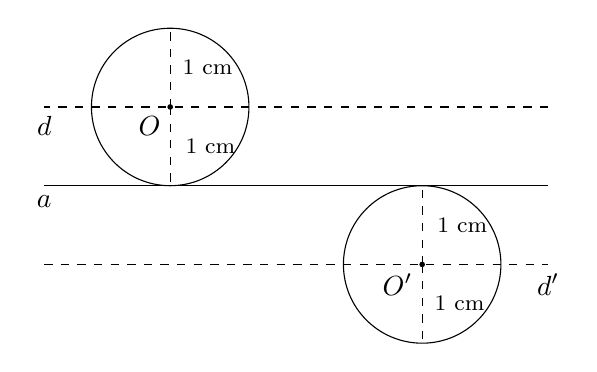
\begin{tikzpicture}[scale=0.8]
	\def\h{1.25}
	\def\hinhgoc(#1,#2,#3,#4){
	\begin{scope}[xscale=#1, yscale=#2]
	\draw (-2,\h) circle (\h){};	
	\draw[fill=black] (-2,\h) circle(1pt) node[below left]{$#3$};
	\draw[dashed](4,\h)--(-4,\h)node[below]{$#4$};	
	\draw[dashed] (-2,\h) -- (-2,2*\h) node [black,midway,right=1pt] {\footnotesize $1$ cm} (-2,\h) -- (-2,0) node [black,midway,right=2pt] {\footnotesize $1$ cm};
	\end{scope}
	}
	\hinhgoc(1,1,O,d)
	\hinhgoc(-1,-1,O',d')
	\draw(4,0)--(-4,0)node[below]{$a$};
	\end{tikzpicture}}	
	}
\end{bt}
%%==========Bài 9
\begin{bt}%[9H2B6]
	Cho góc vuông $Oxy$ và đường tròn tâm $I$ tiếp xúc với hai cạnh của góc $Oxy$ tương ứng tại $M$ và $N$. Biết $OI=a$, tính $OM$.	
	\loigiai
	{\immini{
	Ta có $Ox$ là tiếp tuyến của $(I)$ nên $\widehat{M}=90^\circ$; $Oy$ là tiếp tuyến của $(I)$ nên $\widehat{N}=90^\circ$ và $IM=IN=r$. Do đó tứ giác $OMIN$ là hình vuông, suy ra $OM+MI=\dfrac{a\sqrt{2}}{2}$. Vậy $OM=\dfrac{a\sqrt{2}}{2}$.	}{\begin{tikzpicture}[line join = round, line cap = round,>=stealth,font=\footnotesize,scale=.9]
	\coordinate[label=below:$O$] (O) at (0,0);
	\coordinate[label=below:$x$] (x) at ($(O)+(0:4)$);
	\coordinate[label=left:$y$] (y) at ($(O)+(90:4)$);
	\coordinate(z) at ($(O)+(45:4)$);
	\coordinate[label=above right:$I$] (I) at ($(O)!.5!(z)$);
	\coordinate[label=above left:$M$] (M) at ($(O)!(I)!(y)$);
	\coordinate[label=below:$N$] (N) at ($(O)!(I)!(x)$);
	\tkzDrawCircle(I,M)
	\tkzDrawSegments[dashed](O,I)
	\tkzDrawSegments(O,y O,x I,M I,N)
	\tkzLabelSegment[pos=0.5](O,I){\tiny $a$}
	\tkzLabelSegment[pos=0.5](I,M){\tiny $r$}
	\tkzMarkRightAngles[size=.15](x,O,y O,M,I I,N,O)
	\tkzDrawPoints[color=black,fill=black,size=2pt](O,M,N,I)
	\end{tikzpicture}}
	}
\end{bt}
%%==========Bài 7
\begin{bt}%[9H2K4]
	Cho đường trong $(O)$ và một điểm $A$ nằm ngoài đường tròn $(O)$. Những điểm $M$ sao cho đường thẳng $AM$ không có điểm chung với đường tròn $(O)$ thì nằm ở đâu?
	\loigiai
	{
	\immini{
	Vẽ Đường tròn đường kính $OA$, đường tròn này cắt $(O)$ tại $B$ và $C$. Vì $B$ thuộc đường tròn đường kính $OA$ nên $\widehat{ABO}=90^\circ$. $\Rightarrow OB\perp AB$ $\Rightarrow$ khoảng cách từ $O$ đến đường thẳng $AB$ bằng bán kính $R$ $\Rightarrow AB$ tiếp xúc với $(O)$ tại $C$. Do đó, $M$ nằm trong góc $\widehat{xAB}$ và $\widehat{yAC}$ thì $AM$ không cắt $(O)$.}{\begin{tikzpicture}[line join=round, line cap=round]
	\tikzset{label style/.style={font=\footnotesize}}
	\pgfmathsetmacro\h{1.25}
	\tkzDefPoint(0,0){A}
	\tkzDefShiftPoint[A](0:3*\h){O}
	\tkzDefTangent[from with R=A](O,\h cm)\tkzGetPoints{B}{C}
	\coordinate (O') at ($(A)!1/2!(O)$);
	\coordinate (M) at ($(O')+(120:\h)$);
	\pgfresetboundingbox
	\draw (C)--(A)--(B)--(O)--cycle (A)--(O);
	\draw (O) circle (\h);
	\tkzDrawCircle(O',A)
	\tkzDrawLines[add = 0.5 and 0.5](A,C)
	\tkzDrawLines[add = 0.5 and 0.5](A,B)
	\tkzLabelLine[pos=-.5,above,black](A,C){$x$}
	\tkzLabelLine[pos=-.5,above,black](A,B){$y$}
	\tkzDrawLines[add = 0.5 and 0.5](A,M)
	\tkzDrawPoints[fill=black](O,O',A,B,C)
	\tkzLabelPoints[above left](A,M)
	\tkzLabelPoints[below](O',C)
	\tkzLabelPoints[above](B)
	\tkzLabelPoints[right](O)
	\tkzMarkRightAngles[size=0.15](A,C,O A,B,O)
	\tkzMarkSegments[pos=0.5,mark=|](O',A O',O)
	\end{tikzpicture}}
	}
\end{bt}
%%==========Bài 8
\begin{bt}%[9H2G4]
	Cho tam giác $ABC$ đều cạnh $a$. Gọi $H$ là chân đường cao vẽ từ đỉnh $A$ và $G$ là trọng tâm của tam giác. Lấy một điểm $I$ bất kì bên trong tam giác $CGH$ rồi vẽ đường tròn $(I)$ tiếp xúc với cạnh $AC$. Xác định vị trí tương đối của hai đường thẳng $AB$ và $BC$ với đường tròn $(I)$.
	\loigiai
	{
	\immini{
	Kẻ $ID$, $IE$, $IF$ lần lượt vuông góc với các cạnh $AC$, $BC$, $AB$ của $\triangle ABC$. Vì $I$ nằm trong tam giác $CGH$ và $CG$ là phân giác của $\widehat{BCA}$ nên $\widehat{ICE}<\widehat{ICD}\Rightarrow \sin \widehat{ICE}<\sin \widehat{ICD}$ $\Rightarrow \dfrac{IE}{IC}<\dfrac{ID}{IC}\Rightarrow IE<ID$ nên đường thẳng $BC$ cắt $(I;ID)$ tại hai điểm phân biệt. Tương tự, ta có $IF>ID$ nên đường thẳng $AB$ và $(I;ID)$ không có điểm chung.}{\begin{tikzpicture}[line join=round, line cap=round]
	\tikzset{label style/.style={font=\footnotesize},scale=0.8}
	\pgfmathsetmacro\h{2.5}
	\pgfmathsetmacro\goc{60}
	\tkzDefPoint(0,0){B}
	\tkzDefShiftPoint[B](0:2*\h){C}
	\tkzDefShiftPoint[B](\goc:\h){b}
	\tkzDefShiftPoint[B](10:1.2*\h){I}
	\tkzDefShiftPoint[C](180-\goc:\h){c}
	\coordinate (H) at ($(B)!1/2!(C)$);
	\tkzInterLL(C,c)(B,b)\tkzGetPoint{A}
	\coordinate (M) at ($(A)!1/2!(C)$);
	\tkzInterLL(H,A)(B,M)\tkzGetPoint{G}
	\tkzDefPointBy[projection = onto C--A](I) \tkzGetPoint{D}
	\tkzDefPointBy[projection = onto A--B](I) \tkzGetPoint{F}
	\tkzDefPointBy[projection = onto C--B](I) \tkzGetPoint{E}
	\pgfresetboundingbox
	\tkzDrawPoints[fill=black](A,B,C,H,G,I,M,E,F)
	\draw (A)--(B)--(C)--cycle (A)--(H) (B)--(M) (G)--(C) (F)--(I)--(D) (I)--(E);
	\tkzDrawCircle(I,D)
	\tkzLabelPoints[below](C,B,H,E)
	\tkzLabelPoints[above](A)
	\tkzLabelPoints[left](F,G)
	\tkzLabelPoints[right](M,D)
	\tkzMarkRightAngles[size=0.15](A,H,C I,E,C I,D,C B,M,C I,F,A)
	\end{tikzpicture}}
	}
\end{bt}
%%==========Bài 10
\begin{bt}
	\immini
	{
	Trong hình vẽ bên, $AB$ là tiếp tuyến của đường tròn $(O)$ tại $B$.
	\begin{listEX}[1]
	\item Tính bán kính $r$ của đường tròn $(O)$.
	\item Tính chiều dài cạnh $OA$ của tam giác $ABO$.
	\end{listEX}
	}
	{
	\begin{tikzpicture}[line join = round, line cap = round,>=stealth,font=\footnotesize,scale=0.8]
	\def\r{2}
	\path (0,0) coordinate (O) ({\r+\r*2/3},0) coordinate (A) (\r,0) coordinate (C) ($(O)!.5!(A)$)coordinate (X);
	\path[name path=c'] (X) let \p1=($(X)-(O)$) in circle ({veclen(\x1,\y1)});
	\draw[name path=c] (O) circle (\r);
	\path[name intersections={of=c and c',by={B,B'}}];
	\draw (O)--(C)node[midway,below]{$r$}--(A)node[midway,below]{$2$}--(B)node[above,midway]{$4$}--(O)node[above,midway]{$r$};
	\foreach\i/\j in{O/-90,A/-90,B/90,C/-45}
	\fill[black](\i)circle(1.5pt)node[shift=(\j:2.5mm)]{$\i$};
	\pic[draw, angle radius=5pt]{right angle=A--B--O};
	\end{tikzpicture}
	}
	\loigiai{
	\begin{listEX}[1]
	\item Xét $\triangle OAB$ vuông tại $B$ ta có $OB^2+OA^2=OA^2$ (định lý Pythagore).
	\allowdisplaybreaks
	\begin{eqnarray*}
	OB^2+OA^2&=&OA^2\\
	r^2+4^2&=&(r+2)^2\\
	4r-12&=&0\\
	r=3.
	\end{eqnarray*}
	\noindent Vậy bán kính của $(O)$ bằng $3$.
	\item Ta có $OA=OC+CA=3+2=5$.
	\end{listEX}
	}
\end{bt}
%%==========Bài 11
\begin{bt}
	\immini
	{
	Trong hình bên, $AB=9$, $ BC=12$, $ AC=15$ và $BC$ là đường kính của đường. Chứng minh $AB$ là tiếp tuyến của đường tròn $(O)$
	}
	{
	\begin{tikzpicture}[line join = round, line cap = round,>=stealth,font=\footnotesize,scale=0.8]
	\draw (0,0) coordinate (C)--++(60:4)coordinate (B)node[above left,near end]{$12$}--($(B)!0.75!90:(C)$) coordinate (A)node[above,midway]{$9$}--(C)node[below,near start]{$15$};
	\path ($(C)!.5!(B)$) coordinate (O);
	\draw (O) let \p1=($(O)-(B)$) in circle ({veclen(\x1,\y1)});
	\foreach\i/\j in{C/-135,B/90,A/0,O/180}
	\fill[black](\i)circle(1.5pt)node[shift=(\j:2.5mm)]{$\i$};
	\end{tikzpicture}
	}
	\loigiai{
	Ta có 
	$AB^2=9^2=81$;
	$AC^2=15^2=225$;
	$BC^2=12^2=144$.\\
	Ta có $BC^2=AB^2+BC^2$ ($225=144+81$) nên $\triangle ABC$ vuông tại $B$ (định lý Pythagore đảo).\\
	Ta có $\widehat{OBA}=90^{\circ}$ mà $B\in (O)$ nên $AB$ là tiếp tuyến của đường tròn $(O)$.
	}
\end{bt}
%%==========Bài 12
\begin{bt}
	Cho đường tròn $(O)$ đi qua ba đỉnh $A, B$ và $C$ của một tam giác cân tại $A$. Chứng minh rằng đường thẳng đi qua $A$ và song song với $B C$ là một tiếp tuyến của $(O)$.
	\loigiai{
	\immini{
	Gọi đường thẳng đi qua $A$ và song song với $B C$ và $d$.\\
	Ta có
	$AB=AC$ ($\triangle ABC$ cân tại $A$), $OB=OC=R$. \\
	Suy ra $AO$ là trung trực của $BC$.\\
	Do đó $AO \perp BC$, mà $BC \parallel d$ nên $AO \perp d$.\\
	Ta có $AO \perp d$ tại $A$, suy ra $d$ là tiếp tuyến của đường tròn $(O)$ tại $A$.}{
	\begin{tikzpicture}[scale=0.9, font=\footnotesize, line join=round, line cap=round, >=stealth]
	\coordinate[label=left:$O$] (O) at (0,0);
	\coordinate[label=above:$A$] (A) at ($(0,0)+(90:2cm)$);
	\coordinate[label=below left:$B$] (B) at ($(0,0)+(210:2cm)$);
	\coordinate[label=below right:$C$] (C) at ($(0,0)+(-30:2cm)$);
	\coordinate[label=below:$H$] (H) at ($(C)!0.5!(B)$);
	\draw (O) circle[radius=2cm]; 
	\draw (A)--(B)--(C)--(A)--(H) (-2.5,2)--(2.5,2)node[above]{$d$};
	\foreach \diem in {A,B,O,H}\fill (\diem)circle(1pt); 
	\draw pic[angle radius=2mm,draw=black] {right angle =O--H--B};
	\end{tikzpicture}
	}
	}
\end{bt}
%%==========Bài 13
\begin{bt}
	Cho đường tròn $(O)$ và dây $A B$. Điểm $M$ nằm ngoài đường tròn $(O)$ thoả mãn điểm $B$ nằm trong góc $M A O$ và $\widehat{M A B}=\dfrac{1}{2} \widehat{A O B}$. Chứng minh đường thẳng $M A$ là tiếp tuyến của đường tròn $(O)$.
	\loigiai{\immini{$\widehat{M A B}=\dfrac{1}{2} \widehat{A O B}$ suy ra $\widehat{A O B}=2\widehat{M A B}$.\\ Xét $\triangle AOB$ có $OA=OB$ nên $\triangle AOB$ cân tại $O$.\\
	Suy ra $\widehat{OAB}=\widehat{OBA}$.\\
	Xét $\triangle AOB$ có $\widehat{AOB}\widehat{OAB}+\widehat{OBA}=180^{\circ}$\\
	Hay $2\widehat{MAB}+2\widehat{OAB}=180^{\circ}$ \\
	suy ra $2(\widehat{MAB}+\widehat{OAB})=180^{\circ}$ hay $\widehat{MAB}+\widehat{OAB}=90^{\circ}$\\
	Mà $\widehat{MAB}+\widehat{OAB}=\widehat{OAM}$.\\
	Hay $AO\perp AM$ suy ra $AM$ là tiếp tuyến của $(O)$.}
	{	\begin{tikzpicture}[>=stealth,line join=round,line cap=round,font=\footnotesize,scale=1]
	\def \r{2}
	\path 
	(0,0) coordinate (O)
	(0:\r) coordinate (B)
	(60:\r) coordinate (A)
	($(A)!3!90:(O)$) coordinate (M)
	;
	\draw (O)circle(\r);
	\draw (M)--(A)--(O)--(B)--(A);
	\foreach \x/\y in {M/0,O/-90,A/90,B/0}
	\draw[fill=black] (\x) circle (1.1pt) + (\y:0.3cm) node{$\x$};
	\end{tikzpicture}}
	}
\end{bt}
%%==========Bài 14
\begin{bt}
	\immini{Một người quan sát đặt mắt ở vị trí $A$ có độ cao cách mực nước biển là $A B=5$ m. Cắt bề mặt Trái Đất bởi một mặt phẳng đi qua điểm $A$ và tâm của Trái Đất thì phần chung giữa chúng là một đường tròn lớn tâm $O$ như hình bên. Tầm quan sát tối đa từ vị trí $A$ là đoạn thẳng $A C$, trong đó $C$ là tiếp điểm của tiếp tuyến đi qua $A$ với đường tròn $(O)$. Tính độ dài đoạn thẳng $A C$ (theo đơn vị kilômét và làm tròn kết quả đến hàng phẩn mười), biết bán kính Trái Đất là
	$O B=O C \approx 6400 $ (km)}
	{\begin{tikzpicture}[>=stealth,line join=round,line cap=round,font=\footnotesize,scale=0.8]
	\def \r{2}
	\path 
	(0,0) coordinate (O)
	(60:\r) coordinate (C)
	($(C)!0.7!-90:(O)$) coordinate (A)
	;
	\path[name path=dtron] (O) circle (\r);
	\path[name path=oa] (O)--(A);	
	\path[name intersections={of=dtron and oa, by={B}}];
	\draw (O)circle(\r);
	\draw (O)--(C)--(A)--(O);
	\foreach \x/\y in {A/90,O/-90,C/60,B/235}
	\draw[fill=black] (\x) circle (1.1pt) + (\y:0.3cm) node{$\x$};
	\draw pic[draw, angle radius=2mm, angle eccentricity=1.5]{right angle = A--C--O};
	\end{tikzpicture}}
	\loigiai{
	Vì $AC$ là tiếp tuyến của đường tròn tại $C$ nên $\triangle AOC$ vuông tại $C$.\\
	Áp dụng định lý Py-ta-go cho tam giác $AOC$ vuông tại $C$ ta được\\
	$OA^2=OC^2+AC^2$\\$ AC^2=OA^2-OC^2=6405^2-6400^2=64025$.\\
	Do đó $AC=\sqrt{64025}\approx 253$ (km).
	}
\end{bt}
%%==========Bài 15
\begin{bt}%[9H2B5]
	Cho hệ trục $Oxy$, điểm $A(-1;2)$. Vẽ đường tròn tâm $A$, bán kính $r=\sqrt{5}$, đường tròn này cắt trục tung tại điểm $N$ ($N$ không trùng $O$). Lấy điểm $M(x;0)$ trên trục hoành. Xác định $x$ để $MN$ là tiếp tuyến của $(A;r)$.
	\loigiai
	{
	Ta có $\left(A;\sqrt{5}\right)$ cắt $Oy$ tại $N(0;4)$.\\
	Do đó $AN^2=r^2=5$; $MN^2=x^2+4^2$; $AM^2=(x+1)^2+2^2$.\\
	$MN$ là tiếp tuyến của $(A)$ khi $MN\perp AN\Leftrightarrow AM^2=MN^2+AN^2\Leftrightarrow x=8$.
	}
\end{bt}
%%==========Bài 16
\begin{bt}%[9H2K5]
	Cho nửa đường tròn $(O)$, đường kính $AB$. Từ một điểm $M$ trên đường tròn ta vẽ tiếp tuyến $xy$ với nửa đường tròn. Gọi $H$ và $K$ lần lượt là hình chiếu của $A$ và $B$ trên $xy$. Chứng minh rằng
	\begin{enumerate}
	\item $M$ là trung điểm của $HK$.
	\item Đường tròn đường kính $HK$ tiếp xúc với $AB$.
	\end{enumerate}	
	\loigiai
	{\immini{\vspace*{-1cm}
	\begin{enumerate}
	\item Vì $xy$ là tiếp tuyến nên $OM\perp xy$. Suy ra $AH\parallel BK\parallel OM$. Mà $OA=OB$ nên $MH=MK$.
	\item Vẽ $MD\perp AB$, $D\in AB$, ta có $\widehat{MAH}=\widehat{AMO}$ (so le trong), mà $\widehat{AMO}=\widehat{MAO}$ nên $\widehat{MAH}=\widehat{MAO}$. $\triangle MAH=\triangle MAD$ nên $MH=MD=MK$. Do đó đường tròn đường kính $HK$ đi qua $D$. Ta có $AB\perp MD$ tại $D$ nên $AB$ là tiếp tuyến của đường tròn đường kính $HK$.
	\end{enumerate}}{\begin{tikzpicture}[line join = round, line cap = round,>=stealth,font=\footnotesize,scale=.9]
	\def\ro{2cm}
	\coordinate[label=below:$O$] (O) at (0,0);
	\coordinate[label=below:$B$] (B) at ($(O)+(0:\ro)$);
	\coordinate[label=below:$A$] (A) at ($(O)+(180:\ro)$);
	\coordinate[label=above:$M$] (M) at ($(O)+(110:\ro)$);
	\tkzDefTangent[at=M](O)
	\tkzGetPoint{d}
	\coordinate[label=above:$K$] (K) at ($(d)!(B)!(M)$);
	\coordinate[label=above:$H$] (H) at ($(d)!(A)!(M)$);
	\coordinate[label=below:$D$] (D) at ($(B)!(M)!(A)$);
	\coordinate[label=below:$x$] (x) at ($(K)!1.2!(H)$);
	\coordinate[label=below:$y$] (y) at ($(H)!1.2!(K)$);
	\tkzDrawArc[color=black](O,B)(A)
	\tkzDrawCircle[dashed](M,D)
	\tkzDrawSegments(M,D x,y A,M A,B A,H B,K)
	\tkzMarkRightAngles(A,H,M B,K,M)
	\tkzDrawSegments[dashed](M,O)
	\tkzDrawPoints[color=black,fill=black,size=2pt](A,B,M,H,K,D,O)
	\end{tikzpicture}}
	}
\end{bt}
%%==========Bài 17
\begin{bt}%[9H2K5]
	Cho tam giác $ABC$ vuông tại $A$ ($AB<AC$), đường cao $AH$. Gọi $D$ là điểm đối xứng của $B$ qua $H$. Vẽ $DE \parallel AB$ ($E$ thuộc $AC$). Chứng minh rằng
	\begin{enumerate}
	\item Tam giác $HAE$ cân tại $H$;
	\item $HE$ là tiếp tuyến của đường tròn ngoại tiếp tam giác $CDE$.
	\end{enumerate}	
	\loigiai{
	\immini{
	\begin{enumerate}
	\item Vẽ $HN\parallel AB$. Xét hình thang $ABDE$, ta chứng minh được $NA=NE$ và $HN\perp AE$. Suy ra tam giác $HAE$ cân tại $H$.
	\item Gọi $M$ là trung điểm của $CD$. Vì tam giác $CDE$ vuông tại $E$ nên $M$ là tâm đường tròn ngoại tiếp tam giác $CDE$. Ta có $\widehat{E_2}=\widehat{C}$ và $\widehat{E_1}=\widehat{A_1}$ nên $\widehat{E_2}+\widehat{E_1}=\widehat{C}+\widehat{A_1}=90^\circ\Rightarrow \widehat{HEM}=90^\circ$.
	\end{enumerate}	}{\begin{tikzpicture}[line join = round, line cap = round,>=stealth,font=\footnotesize,scale=1.4]
	\tkzInit[xmin=-.5,ymin=-1.5,xmax=4.5,ymax=2]
	\tkzClip
	\coordinate[label=below:$B$] (B) at (0,0);
	\coordinate[label=below right:$C$] (C) at ($(B)+(0:4)$);
	\tkzDefTriangle[two angles= 65 and 25](B,C)
	\tkzGetPoint{A}
	\node at ($(A)+(90:3mm)$){$A$};
	\tkzDrawPolygon(A,B,C)
	\coordinate[label=below:$H$] (H) at ($(B)!(A)!(C)$);
	\coordinate[label=below right:$D$] (D) at ($(B)!2!(H)$);
	\tkzDefLine[parallel=through D](A,B)
	\tkzGetPoint{d}
	\coordinate[label=above:$E$] (E) at (intersection of A--C and D--d);
	\coordinate[label=above:$N$] (N) at ($(A)!(H)!(C)$);
	\coordinate[label=below:$M$] (M) at ($(D)!.5!(C)$);
	\tkzDrawCircle(M,E)
	\tkzDrawSegments(A,H D,E E,M)
	\tkzDrawSegments[dashed](H,N)
	\tkzMarkRightAngles[size=.2](B,A,C A,H,C)
	\tkzLabelAngles[pos=.3](H,A,N){\tiny $1$}
	\tkzLabelAngles[pos=.3](N,E,H){\tiny $1$}
	\tkzLabelAngles[pos=.4](M,E,C){\tiny $2$}
	\tkzMarkSegments[mark=||,size=2](B,H D,H)
	\tkzMarkSegments[mark=|,size=2](D,M M,C)
	\tkzDrawSegments[add=0 and .3](H,E)
	\tkzDrawPoints[color=black,fill=black,size=2pt](A,B,C,D,H,N,E,M)
	\end{tikzpicture}}	
	}
\end{bt}
%%==========Bài 18
\begin{bt}
	Cho đường tròn $(O)$, điểm $M$ nằm ngoài $(O)$ sao cho $MA$ và $MB$ là hai tiếp tuyến ($A$, $B$ là hai tiếp điểm) thoả mãn $\widehat{AMB}=60^{\circ}$. Biết chu vi tam giác $MAB$ là $18$ cm, tính độ dài dây $AB$.
	\loigiai{
	\immini{
	Ta có $MA=MB$ (tính chất hai tiếp tuyến cắt nhau) mà $\widehat{AMB}=60^{\circ}$ nên $\triangle AMB$ đều.\\
	Khi đó $AB=18:3=6$ cm.
	}{
	\begin{tikzpicture}[line join = round, line cap = round,>=stealth,font=\footnotesize,scale=0.75]
	\def\r{2}
	\pgfmathsetmacro{\a}{\r/sin(30)}
	\path (0,0) coordinate (O) (\a,0) coordinate (M)node[shift=(180:6mm)]{$60^{\circ}$}
	($(O)!.5!(M)$) coordinate (X);
	\path[name path=c'] (X) let \p1=($(X)-(O)$) in circle ({veclen(\x1,\y1)});
	\draw[name path=c] (O) circle (\r);
	\path[name intersections={of=c and c',by={A,B}}];
	\foreach\i/\j in{A/90,B/-90,O/180,M/0}
	\fill[black](\i)circle(1.5pt)node[shift=(\j:2.5mm)]{$\i$};
	\draw (M)--(A)--(O)--(B)--cycle (A)--(B);
	\pic[draw, angle radius=10pt]{angle=A--M--B};
	\pic[draw, angle radius=5pt]{right angle=M--A--O};
	\pic[draw, angle radius=5pt]{right angle=M--B--O};
	\end{tikzpicture}
	}
	}
\end{bt}
%%==========Bài 19
\begin{bt}
	\immini
	{
	Quan sát hình bên. Biết $AB$, $AC$ lần lượt là tiếp tuyến của đường tròn $(O)$ tại $B$, $C$. Tính giá trị của $x$.
	}
	{
	\begin{tikzpicture}[line join = round, line cap = round,>=stealth,font=\footnotesize,scale=1]
	\def\r{1.5}
	\path (0,0) coordinate (O) (-4,0) coordinate (A) ($(O)!.5!(A)$) coordinate (X);
	\draw[name path=c] (O) circle (\r);
	\path[name path=c'] (X) let \p1=($(X)-(O)$) in circle ({veclen(\x1,\y1)});
	\path[name intersections={of=c and c',by={B,C}}];
	\foreach\i/\j in{A/180,B/135,C/-135,O/0}
	\fill[black](\i)circle(1.5pt)node[shift=(\j:2.5mm)]{$\i$};
	\draw (O)--(B)--(A)node[above,midway,rotate=45]{$7x-4$}--(C)node[below,midway]{$3x+8$}--cycle;
	\pic[draw, angle radius=5pt]{right angle=A--B--O};
	\pic[draw, angle radius=5pt]{right angle=A--C--O};
	\end{tikzpicture}
	}
	\loigiai{
	Ta có $AB=AC$ (tính chất hai tiếp tuyến cắt nhau) nên $7x-4=3x+8\Leftrightarrow x=3$.
	}
\end{bt}
%%==========Bài 20
\begin{bt}
	\immini
	{
	Ở hình vẽ bên, $MB$, $MC$ lần lượt là tiếp tuyến của đường tròn $(O)$ tại $B$, $C$; $\widehat{COB}=130^{\circ}$. Tính số đo $\widehat{CMB}$.
	}
	{
	\begin{tikzpicture}[line join = round, line cap = round,>=stealth,font=\footnotesize,scale=1]
	\def\r{1.5}
	\pgfmathsetmacro{\m}{\r/sin(25)}
	\path (0,0) coordinate (O)node[shift=(180:7mm)]{$130^{\circ}$} (-\m,0) coordinate (M) ($(O)!.5!(M)$) coordinate (X);
	\draw[name path=c] (O) circle (\r);
	\path[name path=c'] (X) let \p1=($(X)-(O)$) in circle ({veclen(\x1,\y1)});
	\path[name intersections={of=c and c',by={C,B}}];
	\foreach\i/\j in{M/180,C/135,B/-135,O/0}
	\fill[black](\i)circle(1.5pt)node[shift=(\j:2.5mm)]{$\i$};
	\draw (O)--(B)--(M)--(C)--cycle;
	\pic[draw, angle radius=5pt]{right angle=M--B--O};
	\pic[draw, angle radius=5pt]{right angle=M--C--O};
	\pic[draw, angle radius=5pt]{angle=C--O--B};
	\end{tikzpicture}
	}
	\loigiai{
	Ta có $\widehat{MCO}=\widehat{MBO}=90^{\circ}$ ($MC$, $MB$ lần lượt là tiếp tuyến $(O)$).\\
	Xét tứ giác $MBOC$ ta có
	\begin{eqnarray*}
	\widehat{M}+\widehat{B}+\widehat{O}+\widehat{C}&=&360^{\circ}\\
	\widehat{M}+90^{\circ}+130^{\circ}+90^{\circ}&=&360^{\circ}\\
	\widehat{M}&=&360^{\circ}-90^{\circ}-130^{\circ}-90^{\circ}\\
	\widehat{M}&=&50^{\circ}.
	\end{eqnarray*}
	\noindent
	Vậy $\widehat{CMB}=50^{\circ}$.
	}
\end{bt}
%%==========Bài 21
\begin{bt}
	\immini
	{
	Cho tam giác $ABC$ có đường tròn $(O)$ nằm trong và tiếp xúc với ba cạnh của tam giác. Biết $AM=6$ cm, $BP=3$ cm, $CE=8$ cm. Tính chu vi tam giác $ABC$.
	}
	{
	\begin{tikzpicture}[line join = round, line cap = round,>=stealth,font=\footnotesize,scale=0.7]
	\def\tamnoitiep(#1,#2,#3)(#4){
	\path
	($($(#2)!2mm!(#1)$)!0.5!($(#2)!2mm!(#3)$)$)
	coordinate (#2a)
	($($(#1)!2mm!(#2)$)!0.5!($(#1)!2mm!(#3)$)$)
	coordinate (#1a)
	(intersection of #2-- #2a and
	#1--#1a) coordinate (#4);
	}
	\def\a{11/2}
	\def\b{14/2}
	\def\c{9/2}
	\path (0,0) coordinate (B) (\a,0) coordinate (C);
	\path[name path=c] (B) circle (\c);
	\path[name path=c'] (C) circle (\b);
	\path[name intersections={of=c and c',by={A,D}}];
	\pgfresetboundingbox
	\draw (A)--(B)--(C)--cycle;
	\tamnoitiep(A,B,C)(O)
	\foreach\i/\j in{A/90,B/-135,C/-45,O/45}
	\fill[black](\i)circle(1.5pt)node[shift=(\j:2.5mm)]{$\i$};
	\foreach \i/\j/\l in{A/M/B,A/E/C,C/P/B} \path ($(\i)!(O)!(\l)$) coordinate (\j);
	\draw (O) let \p1=($(M)-(O)$) in circle ({veclen(\x1,\y1)});
	\foreach\i/\j in{A/90,B/-135,C/-45,O/45,M/180,E/45,P/-90}
	\fill[black](\i)circle(1.5pt)node[shift=(\j:2.5mm)]{$\i$};
	\path 
	(A)--(M)node[midway,above,sloped]{$6$cm}
	($(B)!0.5!(P)$)node[below]{$3$cm}
	(E)--(C)node[midway,above,sloped]{$8$cm}
	;
	\end{tikzpicture}
	}
	\loigiai{
	Ta có $BP$, $BM$ lần lượt là hai tiếp tuyến của đường tròn $(O)$. Khi đó $BP=BM=3$ cm (tính chất hai tiếp tuyến cắt nhau).\\
	Tương tự, ta có $AM=AE=6$ cm và $CE=CP=8$ cm.\\
	Khi đó $AB=9$ cm; $BC=11$ cm và $AC=14$ cm là độ dài ba cạnh $\triangle ABC$.\\
	Vậy chu vi $\triangle ABC$ là $9+11+14=34$ cm.
	}
\end{bt}
%%==========Bài 22
\begin{bt}
	Cho góc $x O y$ với đường phân giác $Ot$ và điểm $A$ trên cạnh $O x$, điểm $B$ trên cạnh $O y$ sao cho $O A=O B$. Đường thẳng qua $A$ và vuông góc với $O x$ cắt $O t$ tại $P$. Chứng minh rằng $O A$ và $O B$ là hai tiếp tuyến cắt nhau của đường tròn $(P; P A)$.
	\loigiai{
	\immini{
	Xét $\triangle OAP$ và $\triangle OBP$ ta có:\\
	$OA=OB$ (gt), $OP$ cạnh chung, $\widehat{AOP}=\widehat{BOP}$ ($Ot$ là tia phân giác góc $x O y$).\\
	Suy ra $\triangle OAP=\triangle OBP$ (c.g.c), do đó $\widehat{PAO}=\widehat{PBO}$ (2 góc tương ứng).\\
	Mà $\widehat{PAO}=90^o$ nên $\widehat{PBO}=90^o$.\\
	Ta có $PA \perp AO$ tại $A$ và $PB \perp BO$ tại $B$ nên $OA$, $OB$ là hai tiếp tuyến cắt nhau của $(P; P A)$.}{
	\begin{tikzpicture}[scale=0.7, font=\footnotesize, line join=round, line cap=round, >=stealth]
	\coordinate[label=above right:$P$] (O) at (0,0);
	\coordinate[label=left:$O$] (C) at (-5,0);
	\draw[name path=circleO] (O) circle[radius=2cm];
	\path[name path=circleX] let \p1=($(O)-($(O)!.5!(C)$)$) in ($(O)!.5!(C)$) circle ({veclen(\x1,\y1)});
	\path[name intersections={of= circleX and circleO}] coordinate (A) at (intersection-1) coordinate (B) at (intersection-2);
	\coordinate[label=above:$x$] (X) at ($(A)!-0.5!(C)$);
	\coordinate[label=above:$y$] (Y) at ($(B)!-0.5!(C)$);
	\draw (C)--(A)node[above]{$A$}node[pos=.5,sloped]{|}--(X) (A)--(O)--(B)node[below]{$B$} --(C)node[pos=.5,sloped]{|}--(B)--(Y) (C)--(O)-- ([turn]0:2.5cm)node[above]{$t$};
	\foreach \diem in {O,A,B,C}\fill (\diem)circle(1pt); 
	\draw pic[angle radius=2mm,draw=black] {right angle =O--A--C};
	%	\draw pic[angle radius=2mm,draw=black] {right angle =O--B--C};
	\end{tikzpicture}
	}
	}
\end{bt}
%%==========Bài 23
\begin{bt}
	Cho $S A$ và $S B$ là hai tiếp tuyến cắt nhau của đường tròn $(O)(A$ và $B$ là hai tiếp điểm). Gọi $M$ là một điểm tuỳ ý trên cung nhỏ $A B$. Tiếp tuyến của ($O$) tại $M$ cắt $S A$ tại $E$ và cắt $S B$ tại $F$.
	\begin{enumerate}
	\item Chứng minh rằng chu vi của tam giác $S E F$ bằng $S A+S B$.
	\item Giả sử $M$ là giao điểm của đoạn $S O$ với đường tròn $(O)$. Chứng minh rằng $S E=S F$.
	\end{enumerate}
	\loigiai{
	\begin{enumerate}
	\item 
	\immini{
	Tiếp tuyến tại $A$ và $M$ cắt nhau tại $E$ nên theo tính chất hai tiếp tuyến cắt nhau ta có $AE=EM$.\\
	Tiếp tuyến tại $B$ và $M$ cắt nhau tại $F$ nên theo tính chất hai tiếp tuyến cắt nhau ta có $BF=FM$.\\
	Suy ra chu vi của tam giác $S E F$: $$SE+EF+FS=SE+EM+MF+FS=SE+EA+BF+FS=SA+SB.$$}{
	\begin{tikzpicture}[scale=0.7, font=\footnotesize, line join=round, line cap=round, >=stealth]
	\coordinate[label=right:$O$] (O) at (0,0);
	\coordinate[label=left:$S$] (C) at (-5,0);
	\draw[name path=circleO] (O) circle[radius=2cm];
	\path[name path=circleX] let \p1=($(O)-($(O)!.5!(C)$)$) in ($(O)!.5!(C)$) circle ({veclen(\x1,\y1)});
	\path[name intersections={of= circleX and circleO}] coordinate (A) at (intersection-1) coordinate (B) at (intersection-2);
	\coordinate[label=left:$M$] (M) at ($(0,0)+(160:2cm)$);
	\foreach \diem in {O,A,B,C,M}\fill (\diem)circle(1pt); 
	\draw pic[angle radius=2mm,draw=black] {right angle =O--A--C};
	\draw pic[angle radius=2mm,draw=black] {right angle =O--B--C};
	\draw ($(M)!1!90:(O)$)--($(M)!1.2!-90:(O)$); 
	\draw (C)--(A)node[above]{$A$}--(O)--(B)node[below]{$B$}--(C)--(O) (O)--(M);
	\coordinate (X) at ($(M)!1.2!-90:(O)$);
	\path (intersection of X--M and C--A) coordinate (E) node[above left]{$E$}; 
	\path (intersection of X--M and C--B) coordinate (F) node[below left]{$F$};
	\foreach \diem in {O,A,B,C,M,E,F}\fill (\diem)circle(1pt); 
	\draw pic[angle radius=2mm,draw=black] {right angle =O--M--X};
	\end{tikzpicture}
	}
	\item 
	\immini{
	Tiếp tuyến tại $A$ và $B$ cắt nhau tại $S$ nên theo tính chất hai tiếp tuyến cắt nhau ta có $SO$ là tia phân giác của $\widehat{ASB}$.\\
	Vì $M$ là giao điểm của đoạn $S O$ với đường tròn $(O)$ nên $SM$ là tia phân giác của $\widehat{ASB}$ hay $SM$ là tia phân giác của $\widehat{ESF}$ ($E \in SA$, $F \in SB$).\\
	Vì $M$ là giao điểm của đoạn $S O$ với đường tròn $(O)$ nên $S$, $O$, $M$ thẳng hàng. Mà $OM \perp EF$ suy ra $SM\perp EF$.\\
	Xét $\triangle SEF$ có $SM$ vừa là đường cao, vừa là tia phân giác nên suy ra $\triangle SEF$ cân tại $S$.\\
	Do đó $SE=SF$.}{
	\begin{tikzpicture}[scale=0.85, font=\footnotesize, line join=round, line cap=round, >=stealth]
	\coordinate[label=right:$O$] (O) at (0,0);
	\coordinate[label=left:$S$] (C) at (-5,0);
	\draw[name path=circleO] (O) circle[radius=2cm];
	\path[name path=circleX] let \p1=($(O)-($(O)!.5!(C)$)$) in ($(O)!.5!(C)$) circle ({veclen(\x1,\y1)});
	\path[name intersections={of= circleX and circleO}] coordinate (A) at (intersection-1) coordinate (B) at (intersection-2);
	\coordinate[label=above left:$M$] (M) at ($(0,0)+(180:2cm)$);
	\draw pic[angle radius=2mm,draw=black] {right angle =O--A--C};
	\draw pic[angle radius=2mm,draw=black] {right angle =O--B--C};
	\draw ($(M)!1!90:(O)$)--($(M)!1.2!-90:(O)$); 
	\draw (C)--(A)node[above]{$A$}--(O)--(B)node[below]{$B$}--(C)--(O) (O)--(M) (A)--(B);
	\coordinate (X) at ($(M)!1.2!-90:(O)$);
	\path (intersection of X--M and C--A) coordinate (E) node[above left]{$E$}; 
	\path (intersection of X--M and C--B) coordinate (F) node[below left]{$F$};
	\foreach \diem in {O,A,B,C,M,E,F}\fill (\diem)circle(1pt); 
	\draw pic[angle radius=2mm,draw=black] {right angle =O--M--X};
	\draw pic["$1$", draw=black, angle eccentricity=1.5, angle radius=0.5cm]{angle=O--C--A};
	\draw pic["$2$", draw=black, angle eccentricity=1.5, angle radius=0.45cm]{angle=B--C--O};
	\end{tikzpicture}
	}
	\end{enumerate}	
	}
\end{bt}
%%==========Bài 24
\begin{bt}
	Cho đường tròn $(O;R)$ có đường kính $AB$. Vẽ dây $AC$ sao cho $AC=R$. Gọi $I$ là trung điểm của dây $AC$. Đường thẳng $OI$ cắt tiếp tuyến $Ax$ tại $M$. Chứng minh rằng
	\begin{listEX}[1]
	\item $\widehat{ACB}$ có số đo bằng $90^{\circ}$, từ đó suy ra độ dài của $BC$ theo $R$;
	\item $OM$ là tia phân giác của $\widehat{COA}$;
	\item $MC$ là tiếp tuyến của đường tròn $(O;R)$.
	\end{listEX}
	\loigiai{
	\begin{center}
	\begin{tikzpicture}[line join = round, line cap = round,>=stealth,font=\footnotesize,scale=1]
	\def\r{2}
	\path (0,0) coordinate (O) (-\r,0) coordinate (A) (\r,0) coordinate (B) ($(O)!1!-60:(A)$) coordinate (C) ($(A)!.5!(C)$) coordinate (I) ($(A)!0.8!90:(B)$)coordinate (x) (intersection of A--x and O--I) coordinate (M);
	\draw (O) circle (\r);
	\draw (C)--(A)--(B)--cycle (A)--(x)node[left]{$x$} (O)--(M)--(C)--(O);
	\foreach\i/\j in{O/-90,A/180,B/0,C/135,I/-455,M/180}
	\fill[black](\i)circle(1.5pt)node[shift=(\j:2.5mm)]{$\i$};
	\pic[draw, angle radius=5pt]{right angle=x--A--B};
	\end{tikzpicture}
	\end{center}
	\begin{listEX}[1]
	\item $\triangle ACO$ đều ($AC=AO=CO=R$) nên $\widehat{ACO}=\widehat{COA}=60^{\circ}$ $$\Rightarrow \widehat{COB}=180^{\circ}-60^{\circ}=120^{\circ}.$$
	Xét $\triangle COB$ cân tại $O$ ta có $\widehat{OCB}=\widehat{OBC}=\dfrac{180^{\circ}-120^{\circ}}{2}=30^{\circ}$.\\
	Vậy $\widehat{ACB}=60^{\circ}+30^{\circ}=90^{\circ}$.\\
	Xét $\triangle ABC$ vuông tại $C$ ta có $BC=AB\cdot \cos(30)=\dfrac{\sqrt{3}}{2}R$.
	\item Ta có $I$ là trung điểm $AC$ mà $OC=OA=R$ nên $OI$ là trung trực đoạn thẳng $AC$.\\
	Do $\triangle OAC$ đều nên $OI$ là phân giác $\widehat{COA}$.
	\item Xét $\triangle AOM$ và $\triangle COM$ ta có 
	$\heva{& OA=OC=R \\ & \widehat{AOM}=\widehat{COM}\\& \widehat{MO}\,\text{chung}}\Rightarrow \triangle AOM = \triangle COM$ (c$-$g$-$c).\\
	Khi đó $\widehat{MCO}=\widehat{MAO}=90^{\circ}$ (góc tương ứng bằng nhau).\\
	Mà $C \in (O)$ nên $MC$ là tiếp tuyến của đường tròn $(O;R)$.
	\end{listEX}
	}
\end{bt}
%%==========Bài 25
\begin{bt}
	Cho đường tròn $(O;5\text{cm})$, diểm $M$ nằm ngoài $(O)$ sao cho hai tiếp tuyến $MA$ và $MB$ ($A$, $B$ là hai tiếp điểm) vuông góc với nhau tại $M$.
	\begin{listEX}[1]
	\item Tính độ dài của $MA$ và $MB$.
	\item Qua giao điểm $I$ của đoạn thẳng $MO$ và đường tròn $(O)$, vẽ một tiếp tuyến cắt $OA$, $OB$ lần lượt tại $C$, $D$. Tính độ dài của $CD$.
	\end{listEX}
	\loigiai{
	\begin{center}
	\begin{tikzpicture}[line join = round, line cap = round,>=stealth,font=\footnotesize,scale=1]
	\def\r{2}
	\pgfmathsetmacro{\a}{\r/sin(45)}
	\path (0,0) coordinate (O) (\a,0) coordinate (M) 
	($(O)!.5!(M)$) coordinate (X) (\r,0) coordinate (I) ($(I)!1.2!90:(O)$)coordinate (x) ($(I)!1.2!-90:(O)$)coordinate (x');
	\path[name path=c'] (X) let \p1=($(X)-(O)$) in circle ({veclen(\x1,\y1)});
	\draw[name path=c] (O) circle (\r);
	\path[name intersections={of=c and c',by={A,B}}];
	\path (intersection of O--A and I--x) coordinate (C) (intersection of O--B and I--x') coordinate (D);
	\foreach\i/\j in{A/90,B/-90,O/-90,M/0,I/-135,D/-45,C/45}
	\fill[black](\i)circle(1.5pt)node[shift=(\j:2.5mm)]{$\i$};
	\draw (O)--(A)--(M)--(B)--cycle (C)--(D) (A)--(C) (B)--(D) (O)--(M);
	\pic[draw, angle radius=5pt]{right angle=A--M--B};
	\pic[draw, angle radius=5pt]{right angle=O--A--M};
	\pic[draw, angle radius=5pt]{right angle=O--B--M};
	\pic[draw, angle radius=5pt]{right angle=O--I--C};
	\end{tikzpicture}
	\end{center}
	\begin{listEX}[1]
	\item Ta có $MA$; $MB$ là tiếp tuyến của $(O)$ nên $\widehat{OAM}=\widehat{OBM}=90^{\circ}$.\\
	Mặt khác $\widehat{AMB}=90^{\circ}$ (gt) nên tứ giác $OABM$ là hình chữ nhật.\\
	Do $MA=MB$ (tính chất hai tiếp tuyến cắt nhau) nên tứ giác $OABM$ là hình vuông.\\
	Vậy $MA=MB=OA=OB=R=5$ cm.
	\item Ta có $CD$ là tiếp tuyến của $(O)$ nên $OI\perp CD$.\\
	Xét $\triangle IOC$ và $\triangle AOM$ ta có\\
	$\heva{& \widehat{I}=\widehat{A}=90^{\circ} \\ & IO=AO=R\\& \widehat{O}\,\text{chung}}\Rightarrow \triangle IOC=\triangle AOM$ (g $-$ c $-$ g).\\
	Khi đó $IO=AM=5$ cm.\\
	Tương tự, ta có $ID=BM=5$ cm.\\
	Khi đó $CD=CI+ID=5+5=10$ cm.
	\end{listEX}
	}
\end{bt}
%%==========Bài 26
\begin{bt}
	Cho đường tròn $(O)$ và điểm $M$ nằm ngoài đường tròn. Hai đường thẳng $c$, $d$ đi qua $M$ lần lượt tiếp xúc với $(O)$ tại $A$, $B$. Tia phân giác của góc $M A B$ cắt $M O$ tại $I$. Chứng minh điểm $I$ cách đều ba đường thẳng $M A$, $M B$ và $A B$.
	\loigiai{
	\immini{
	$c$, $d$ đi qua $M$ lần lượt tiếp xúc với $(O)$ tại $A$, $B$. Do đó $c$, $d$ là hai tiếp tuyến nên $MO$ là tia phân giác của góc $AMB$.\\
	Lại có $AI$ là tia phân giác của góc $MAB$.\\
	Mà ba đường phân giác của một tam giác đi qua một điểm và điểm đó cách đều ba cạnh của tam giác. Do đó $I$ cách đều ba đường thẳng $MA$, $MB$ và $AB$. }
	{\begin{tikzpicture}[>=stealth,line join=round,line cap=round,font=\footnotesize,scale=0.7]
	\def \r{2}
	\path 
	(0,0) coordinate (O)
	(65:\r) coordinate (A)
	(-65:\r) coordinate (B)
	($(A)!2!90:(O)$) coordinate (x)
	($(B)!2!-90:(O)$) coordinate (y)
	($(A)!0.3!180:(x)$) coordinate (c)
	($(B)!0.3!180:(y)$) coordinate (d)
	(intersection of A--x and B--y) coordinate (M)
	($(A)!1!-35:(M)$) coordinate (e)
	(intersection of M--O and A--e) coordinate (I)
	;
	\draw (O)circle(\r);
	\draw (M)--(B)--(O)--(A)--(M)(A)--(c) (A)--(B)--(d) (M)--(O) (A)--(I);
	\foreach \x/\y in {A/90,O/180,M/0,B/-90,I/-110}
	\draw[fill=black] (\x) circle (1.1pt) + (\y:0.3cm) node{$\x$};
	\foreach \x/\y in {c/90,d/-90}
	\draw[fill=black] (\x) circle (0pt) + (\y:0.3cm) node{$\x$};
	\end{tikzpicture}}
	}
\end{bt}
%%==========Bài 27
\begin{bt}
	\immini{Cho đường tròn $(O; R)$ đường kính $A B$ và các đường thẳng $m$, $n$, $p$ lần lượt tiếp xúc với đường tròn tại $A$, $B$, $C$. Chứng minh:
	\begin{enumerate}
	\item $A D+B E=D E$;
	\item $\widehat{C O D}=\dfrac{1}{2} \widehat{C O A}$ và $\widehat{C O E}=\dfrac{1}{2} \widehat{C O B}$;
	\item Tam giác $O D E$ vuông;
	\item $\dfrac{O D \cdot O E}{D E}=R$.
	\end{enumerate}}
	{\begin{tikzpicture}[>=stealth,line join=round,line cap=round,font=\footnotesize,scale=0.7]
	\def \r{2}
	\path 
	(0,0) coordinate (O)
	(180:\r) coordinate (A)
	(0:\r) coordinate (B)
	(110:\r) coordinate (C)
	($(C)!1.7!90:(O)$) coordinate (p')
	($(C)!1.5!-90:(O)$) coordinate (p)
	($(A)!0.8!90:(B)$) coordinate (m')
	($(B)!1.3!-90:(A)$) coordinate (n')
	($(A)!0.6!180:(m')$) coordinate (m)
	($(B)!0.45!180:(n')$) coordinate (n)
	(intersection of A--m and C--p) coordinate (D)
	(intersection of C--p' and B--n) coordinate (E)
	;
	\draw (O)circle(\r);
	\draw (p)--(p')(m')--(m)(n')--(n) (C)--(O)--(A) (O)--(B) (D)--(O)--(E);
	\foreach \x/\y in {A/180,O/-90,B/0,C/90,D/130,E/70}
	\draw[fill=black] (\x) circle (1.1pt) + (\y:0.3cm) node{$\x$};
	\foreach \x/\y in {p/90,m/180,n/0}
	\draw[fill=black] (\x) circle (0pt) + (\y:0.3cm) node{$\x$};
	\end{tikzpicture}}
	\loigiai{
	\begin{enumerate}
	\item Đường thẳng $m$, $n$, $p$ tiếp xúc với đường tròn tại các điểm $A$, $B$, $C$. Do đó $m$, $n$, $p$ là các tiếp tuyến của đường tròn.\\
	Hai tiếp tuyến $p$ và $m$ cắt nhau tại $D$, suy ra $DA=DC$\, \hfill{(1)}.\\
	Hai tiếp tuyến $n$ và $p$ cắt nhau tại $E$, suy ra $EB=EC$\, \hfill{(2)}.\\
	Khi đó $DE=DC+CE=DA+EB$.\\
	Vậy $A D+B E=D E$.
	\item 
	Hai tiếp tuyến $p$ và $m$ cắt nhau tại $D$, suy ra $OD$ là tia phân giác của góc $AOC$. \\
	Hay $\widehat{C O D}=\dfrac{1}{2} \widehat{C O A}$.\\
	Hai tiếp tuyến $n$ và $p$ cắt nhau tại $E$, suy ra $OE$ là tia phân giác của góc $BOC$.\\ Hay $\widehat{C O E}=\dfrac{1}{2} \widehat{C O B}$.\\
	\item Ta có $\widehat{AOD}+\widehat{DOC}+\widehat{COE}+\widehat{EOB}=180^{\circ}$.\\
	$OD$ là tia phân giác của góc $AOC$\\
	$OE$ là tia phân giác của góc $BOC$\\
	nên $2\widehat{DOC}+2\widehat{COE}=180^{\circ}$ hay $\widehat{DOE}=90^{\circ}$.\\
	Do đó tam giác $O D E$ vuông;
	\item $\triangle DOE$ vuông tại $O$ có $OC$ là đường cao.\\
	Áp dụng hệ thức lượng trong $\triangle DOE$ ta được $OD\cdot OE=OC\cdot DE$\\Suy ra $OC=\dfrac{O D \cdot O E}{D E}=R$.
	\end{enumerate}
	}
\end{bt}
%%==========Bài 28
\begin{bt}%[9H2B6]
	Cho đường tròn $(O;R)$. Từ một điểm $A$ cách $O$ một khoảng $2R$ ta vẽ hai tiếp tuyến $AB$, $AC$ ($B$, $C$ là tiếp điểm). Chứng minh rằng $ABC$ là tam giác đều.	
	\loigiai{
	\immini{
	Vì $AB$, $AC$ là hai tiếp tuyến nên $AB=AC$ và $\widehat{A_1}=\widehat{A_2}$. Ta có $OB\perp AB$. Xét tam giác $AOB$ vuông tại $B$ có $OB=\dfrac{1}{2}OA$ nên $\widehat{A_1}=30^\circ$, suy ra $\widehat{BAC}=60^\circ$. Tam giác $ABC$ cân tại $A$, lại có $\widehat{A}=60^\circ$ nên là tam giác đều.}{\begin{tikzpicture}[line join = round, line cap = round,>=stealth,font=\footnotesize,scale=.7]
	\def\ro{2cm}
	\coordinate[label=right:$O$] (O) at (0,0);
	\coordinate[label=left:$A$] (A) at ($(O)+(180:2.5*\ro)$);
	\draw (O) circle(\ro);
	\coordinate (N) at ($(O)+(10:\ro)$);
	\tkzDefTangent[from=A](O,N)
	\tkzGetPoints{B}{C}
	\node at ($(B)+(110:3mm)$){$B$};
	\node at ($(C)+(-90:3mm)$){$C$};
	\tkzDrawSegments[add=0 and .3](A,B A,C)
	\tkzDrawSegments(O,A B,C)
	\tkzDrawSegments[dashed](O,B)
	\tkzMarkSegments[mark=|,size=2](A,B A,C)
	\tkzLabelAngles[pos=.4](O,A,B){\tiny $1$}
	\tkzLabelAngles[pos=.4](C,A,O){\tiny $2$}
	\tkzMarkRightAngles(A,B,O)
	\tkzDrawPoints[color=black,fill=black,size=2pt](A,B,C,O)
	\end{tikzpicture}}	
	}
\end{bt}
%%==========Bài 29
\begin{bt}%[9H2K6]
	Cho tứ giác $ABCD$ ngoại tiếp đường tròn $(O)$ (bốn cạnh $AB$, $BC$, $CD$ và $DA$ đều tiép xúc với $(O)$). Chứng minh rằng $AB+CD=AD+BC$. 	
	\loigiai{
	\immini{
	Vì tứ giác $ABCD$ ngoại tiếp đường tròn $(O)$ nên $AB$, $BC$, $CD$ và $DA$ tiếp xúc với $(O)$. Gọi các tiếp điểm lần lượt tại $M$, $N$, $P$, $Q$. Vì $AM$, $AQ$ là tiếp tuyến của $(O)$ nên $AM=AQ$. Tương tự ta có $BM=BN$, $CN=CP$, $DP=DQ$. Suy ra $AB+CD=AM+MB+CP=DP=AQ+BN+CN+DQ=(AQ+DQ)+(BN+NC)=AD+BC$ (ĐPCM).	}{\begin{tikzpicture}[line join = round, line cap = round,>=stealth,
	font=\footnotesize,scale=.45]
	%, Hình 146
	\tkzDefPoints{0/0/O}
	\def \r{3};
	\coordinate (q) at ($(O)+(\r,0)$);
	\tkzDrawCircle[radius](O,q)
	\coordinate (a) at ($(O)+(0,-\r)$);
	\def\x{20}
	\tkzDefPointBy[rotation = center O angle \x+140](q) \tkzGetPoint{b}
	\tkzDefPointBy[rotation = center O angle \x+60](q) \tkzGetPoint{c}
	\tkzDefPointBy[rotation = center O angle \x](q) \tkzGetPoint{d}
	\foreach \u in {a,b,c,d}
	{\tkzDefTangent[at=\u](O)
	\tkzGetPoint{\u'}}	
	\tkzInterLL(a,a')(b,b') \tkzGetPoint{D}
	\tkzInterLL(b,b')(c,c') \tkzGetPoint{A}
	\tkzInterLL(c,c')(d,d') \tkzGetPoint{B}
	\tkzInterLL(d,d')(a,a') \tkzGetPoint{C}
	\coordinate (Q) at ($(b)+(0,0)$);
	\coordinate (M) at ($(c)+(0,0)$);
	\coordinate (P) at ($(a)+(0,0)$);
	\coordinate (N) at ($(d)+(0,0)$);
	\pgfresetboundingbox
	\tkzDrawPolygon(A,B,C,D)
	\tkzDrawPoints[fill=black](O,a,b,c,d,A,B,C,D)
	\tkzLabelPoints[above](A,B,M)
	\tkzLabelPoints[left](D,Q)
	\tkzLabelPoints[right](C,N)
	\tkzLabelPoints[below left](O)
	\tkzLabelPoints[below](P)
	\end{tikzpicture}}
	}
\end{bt}
%%==========Bài 30
\begin{bt}%[9H2G6]
	Cho đường tròn $(O;R)$ và đường thẳng $xy$ không giao nhau. Trên $xy$ lấy điểm $M$. Từ $M$ vẽ các tiếp tuyến $MA$, $MB$ với đường tròn $(O;R)$ ($A$, $B$ là các tiếp điểm). Vẽ $OH\perp xy$ ($H\in xy$). Dây $AB$ cắt $OH$ tại $E$, cắt $OM$ tại $F$. Chứng minh rằng
	\begin{enumerate}
	\item $OE\cdot OH=OF\cdot OM$;
	\item $OE\cdot OH=R^2$, từ đó suy ra dây $AB$ luôn đi qua một điểm cố định là điểm $E$.
	\end{enumerate}	
	\loigiai{
	\immini{ \vspace*{-0.5cm}	
	\begin{enumerate}
	\item Ta có $MA=MB$ và $\widehat{M_1}=\widehat{M_2}$ suy ra $MO\perp AB$. Tam giác $FOE$ đồng dạng với tam giác $HOM$ nên\\ $\dfrac{OE}{OM}=\dfrac{OF}{OH}\Rightarrow OE\cdot OH=OF\cdot OM$. \tagEX{1}	
	\item Ta có $OA\perp MA$ (tính chất tiếp tuyến). Tam giác $AOM$ đồng dạng với tam giác $FAM$, từ đó ta có $OA^2=OF\cdot OM$. \tagEX{2}
	Từ $(1)$ và $(2)$ suy ra $OE\cdot OH=OA^2=R^2$. Suy ra $OE=\dfrac{R^2}{OH}$ (không đổi). Điểm $E$ nằm trên tia $OH$ cố định, mà $OE$ không đổi nên $E$ là điểm cố định.
	\end{enumerate}}{\begin{tikzpicture}[line join = round, line cap = round,>=stealth,font=\footnotesize,scale=.65]
	\coordinate[label=below:$x$] (x) at (0,0);
	\coordinate[label=below:$y$] (y) at ($(x)+(0:5)$);
	\coordinate[label=below:$M$] (M) at ($(x)!.3!(y)$);
	\coordinate[label=below:$H$] (H) at ($(x)!.6!(y)$);
	\coordinate[label=right:$O$] (O) at ($(H)+(90:5)$);
	\coordinate(o) at ($(O)+(90:2.5)$);
	\tkzDrawCircle(O,o)
	\tkzDefTangent[from=M](O,o)
	\tkzGetPoints{A}{B}
	\coordinate[label=below left:$F$] (F) at (intersection of M--O and A--B);
	\coordinate[label=above right:$E$] (E) at (intersection of O--H and A--B);
	\node at ($(A)+(180:3mm)$){$A$};
	\node at ($(B)+(-30:3mm)$){$B$};
	\tkzMarkSegments[mark=|,size=2](M,A M,B)
	\tkzMarkRightAngles(O,A,M O,H,y M,F,B)
	\tkzMarkAngle[arc=l,size=1](O,M,A)
	\tkzMarkAngle[arc=l,size=1](B,M,O)
	\tkzDrawSegments[add=0 and .3](M,A M,B)
	\tkzDrawSegments(x,y A,B O,H)
	\tkzDrawSegments[dashed](M,O O,A)
	\tkzLabelAngles[pos=.4](O,M,A){\tiny $1$}
	\tkzLabelAngles[pos=.4](B,M,O){\tiny $2$}
	\tkzDrawPoints[color=black,fill=black,size=2pt](A,B,E,F,H,O,M)
	\end{tikzpicture}}
	}
\end{bt}
%%==========Bài 31
\begin{bt}%[9H2K5]
	Cho $(O;R)$ và điểm $A$ cố định nằm ngoài đường tròn. Qua $A$ vẽ đường thẳng $d$ cắt $(O;R)$ tại $B$, $C$ ($AB\le AC$), vẽ tiếp tuyến $AM$ với $(O;R)$ (với $M$ là tiếp điểm). Chứng minh rằng $AB+AC\ge 2AM$.	
	\loigiai{
	\immini{
	Kẻ $OH\perp BC$ tại $H$ nên $HB=HC$ suy ra $AB+AC=2AH$. Ta sẽ chứng minh $AH\ge AM$.
	Áp dụng định lí Py-ta-go vào tam giác vuông $AOH$ và tam giác vuông $AOM$, ta có $OA^2=OH^2+AH^2$, $OA^2=OM^2+AM^2$. Vì $d$ có điểm chung với đường tròn $(O)$ nên $OH\le R=OM\Rightarrow OH^2\le OM^2$ mà $OH^2+AH^2=OM^2+AM^2$ nên $AH^2\ge AM^2$ hay $AH\ge AM$ nên $AB+AC\ge 2AM$. Dấu $''=''$ xảy ra $\Leftrightarrow OH=R\Leftrightarrow d$ tiếp xúc với $(O)$.	}{\begin{tikzpicture}[line join = round, line cap = round,>=stealth,scale=0.9]
	\tkzDefPoints{0/0/O}
	%, Hình 145
	\def \R{2}; %Bán kính
	\draw (O) circle (\R);
	\coordinate (A) at ($(O)+(-3*\R,0)$);
	\tkzDefTriangle[two angles = -15 and -135](A,O) \tkzGetPoint{d}
	\tkzDefTangent[from with R = A](O,\R cm)	\tkzGetPoints{M}{N}
	\tkzInterLC(A,d)(O,M) \tkzGetPoints{C}{B}
	\tkzDefPointBy[projection = onto B--C](O) \tkzGetPoint{H}
	\pgfresetboundingbox
	\tkzDrawPolygon(A,M,O)
	\tkzDrawSegments(A,O A,d O,H)
	\tkzDrawPoints[fill=black](O,A,M,B,C)
	\tkzLabelPoints[above](M,d)
	\tkzLabelPoints[below left](B)
	\tkzLabelPoints[below](C,H)
	\tkzLabelPoints[left](A)
	\tkzLabelPoints[right](O)
	\path (O)--(M) node[above,midway,sloped]{$R$};
	\tkzMarkRightAngles[size=.2](O,M,A O,H,C)
	\tkzMarkSegments[mark=|](H,B H,C)
	\end{tikzpicture}}	
	}
\end{bt}
%%==========Bài 32
\begin{bt}%[9H2G6]
	Cho hình thang cân $ABCD$ ($AB\parallel CD$) ngoại tiếp đường tròn $(O;R)$. Tìm giá trị nhỏ nhất của tổng $AB+CD$ theo $R$.	
	\loigiai{
	\immini{
	Dễ thấy $\widehat{O_1}=\widehat{O_2}$; $\widehat{O_3}=\widehat{O_4}$ $\Rightarrow \widehat{O_2}+\widehat{O_3}=90^\circ$. Áp dụng hệ thức $h^2=b'\cdot c'$ vào tam giác vuông $AOD$, ta có $OF^2=AF\cdot FD=AE\cdot DK=\dfrac{AB}{2}\cdot \dfrac{CD}{2}$ $\Rightarrow AB\cdot CD=4OF^2=4R^2$ ( vì $AF=AE=\dfrac{1}{2}AB$, $DF=DK=\dfrac{1}{2}DC$ và $OF=R$).\\
	Áp dụng bất đẳng thức Cô-si, ta có $AB+CD\ge 2 \sqrt{AB\cdot CD}=2\sqrt{4R^2}=4R$. Dấu $''=''$ xảy ra khi và chỉ khi $AB=CD=2R$. Vậy $AB+CD$ nhỏ nhất bằng $4R$ khi $ABCD$ là hình vuông.}{\begin{tikzpicture}[line join = round, line cap = round,>=stealth,
	font=\footnotesize,scale=.6]
	%, Hình 147
	\tkzDefPoints{0/0/O}
	\def \r{3};
	\coordinate (q) at ($(O)+(\r,0)$);
	\tkzDrawCircle[radius](O,q)
	\coordinate (a) at ($(O)+(0,-\r)$);
	\def\x{20}
	\tkzDefPointBy[rotation = center O angle \x+140](q) \tkzGetPoint{b}
	\tkzDefPointBy[rotation = center O angle 180](a) \tkzGetPoint{c}
	\tkzDefPointBy[rotation = center O angle \x](q) \tkzGetPoint{d}
	\foreach \u in {a,b,c,d}
	{\tkzDefTangent[at=\u](O)
	\tkzGetPoint{\u'}}	
	\tkzInterLL(a,a')(b,b') \tkzGetPoint{D}
	\tkzInterLL(b,b')(c,c') \tkzGetPoint{A}
	\tkzInterLL(c,c')(d,d') \tkzGetPoint{B}
	\tkzInterLL(d,d')(a,a') \tkzGetPoint{C}
	\coordinate (F) at ($(b)+(0,0)$);
	\coordinate (E) at ($(c)+(0,0)$);
	\coordinate (K) at ($(a)+(0,0)$);
	\pgfresetboundingbox
	\tkzDrawPolygon(A,B,C,D)
	\tkzDrawPoints[fill=black](O,a,b,c,d,A,B,C,D)
	\tkzLabelPoints[above](A,B,E)
	\tkzDrawSegments[dashed](E,K O,F O,A O,D)
	\tkzLabelPoints[left](D,F)
	\tkzLabelPoints[right](C,O)
	\tkzLabelPoints[below](K)
	\tkzLabelAngles[pos=-1,rotate=0](A,O,E){$1$}
	\tkzLabelAngles[pos=-1,rotate=0](F,O,A){$2$}
	\tkzLabelAngles[pos=-1,rotate=0](D,O,F){$3$}
	\tkzLabelAngles[pos=-1,rotate=0](K,O,D){$4$}
	\tkzMarkRightAngles[size=0.2](A,E,O O,K,D O,F,D)
	\end{tikzpicture}}	
	}
\end{bt}